\documentclass[twoside, 12pt]{article}
%\usepackage{lmodern}

\usepackage[inner=1.5in, outer=1in, 
top=1in, bottom=1in, headsep=0.5in, footskip=0.5in]{geometry}
%\setlength{\oddsidemargin}{1.5in}
%\setlength{\evensidemargin}{1in}
\usepackage{amssymb,amsmath}


\usepackage{fancyhdr}
\pagestyle{fancy}
\renewcommand{\headrulewidth}{0pt}
\fancyhead[L,R,C]{}
\fancyfoot[RE,LO]{RStudio Instructions}
\fancyfoot[C]{Reed College Bio 101/102: Quantitative}
\fancyfoot[RO,LE]{\thepage}

%\usepackage{scrpage2}
%\pagestyle{scrheadings}           % use following definitions for header/footer
% definitions/configuration for the header
%\rehead[]{}        % equal page, right position (inner) 
%\lohead[]{}        % odd   page, left  position (inner) 
%\lehead[]{} % equal page, left (outer) position
%\rohead[]{}
% definitions/configuration for the footer
%\cefoot[]{center of the footer!}  % equal page, center position
%\cofoot[\pagemark]{\pagemark}     % odd   page, center position

\usepackage{ifxetex,ifluatex}
\usepackage{fixltx2e} % provides \textsubscript
\ifnum 0\ifxetex 1\fi\ifluatex 1\fi=0 % if pdftex
  \usepackage[T1]{fontenc}
  \usepackage[utf8]{inputenc}
\else % if luatex or xelatex
  \ifxetex
    \usepackage{mathspec}
    \usepackage{xltxtra,xunicode}
  \else
    \usepackage{fontspec}
  \fi
  \defaultfontfeatures{Mapping=tex-text,Scale=MatchLowercase}
  \newcommand{\euro}{€}
\fi
% use upquote if available, for straight quotes in verbatim environments
\IfFileExists{upquote.sty}{\usepackage{upquote}}{}
% use microtype if available
\IfFileExists{microtype.sty}{%
\usepackage{microtype}
\UseMicrotypeSet[protrusion]{basicmath} % disable protrusion for tt fonts
}{}

\ifxetex
  \usepackage[setpagesize=false, % page size defined by xetex
              unicode=false, % unicode breaks when used with xetex
              xetex]{hyperref}
\else
  \usepackage[unicode=true]{hyperref}
\fi
\hypersetup{breaklinks=true,
            bookmarks=true,
            pdfauthor={},
            pdftitle={RStudio Instructions},
            colorlinks=true,
            citecolor=blue,
            urlcolor=blue,
            linkcolor=magenta}%,
  %          pdfborder={0 0 0}}
\urlstyle{same}  % don't use monospace font for urls
\usepackage{color}
\usepackage{fancyvrb}
\newcommand{\VerbBar}{|}
\newcommand{\VERB}{\Verb[commandchars=\\\{\}]}
\DefineVerbatimEnvironment{Highlighting}{Verbatim}{commandchars=\\\{\}}
% Add ',fontsize=\small' for more characters per line
\usepackage{framed}
\definecolor{shadecolor}{RGB}{248,248,248}
\newenvironment{Shaded}{\begin{snugshade}}{\end{snugshade}}
\newcommand{\KeywordTok}[1]{\textcolor[rgb]{0.13,0.29,0.53}{\textbf{{#1}}}}
\newcommand{\DataTypeTok}[1]{\textcolor[rgb]{0.13,0.29,0.53}{{#1}}}
\newcommand{\DecValTok}[1]{\textcolor[rgb]{0.00,0.00,0.81}{{#1}}}
\newcommand{\BaseNTok}[1]{\textcolor[rgb]{0.00,0.00,0.81}{{#1}}}
\newcommand{\FloatTok}[1]{\textcolor[rgb]{0.00,0.00,0.81}{{#1}}}
\newcommand{\ConstantTok}[1]{\textcolor[rgb]{0.00,0.00,0.00}{{#1}}}
\newcommand{\CharTok}[1]{\textcolor[rgb]{0.31,0.60,0.02}{{#1}}}
\newcommand{\SpecialCharTok}[1]{\textcolor[rgb]{0.00,0.00,0.00}{{#1}}}
\newcommand{\StringTok}[1]{\textcolor[rgb]{0.31,0.60,0.02}{{#1}}}
\newcommand{\VerbatimStringTok}[1]{\textcolor[rgb]{0.31,0.60,0.02}{{#1}}}
\newcommand{\SpecialStringTok}[1]{\textcolor[rgb]{0.31,0.60,0.02}{{#1}}}
\newcommand{\ImportTok}[1]{{#1}}
\newcommand{\CommentTok}[1]{\textcolor[rgb]{0.56,0.35,0.01}{\textit{{#1}}}}
\newcommand{\DocumentationTok}[1]{\textcolor[rgb]{0.56,0.35,0.01}{\textbf{\textit{{#1}}}}}
\newcommand{\AnnotationTok}[1]{\textcolor[rgb]{0.56,0.35,0.01}{\textbf{\textit{{#1}}}}}
\newcommand{\CommentVarTok}[1]{\textcolor[rgb]{0.56,0.35,0.01}{\textbf{\textit{{#1}}}}}
\newcommand{\OtherTok}[1]{\textcolor[rgb]{0.56,0.35,0.01}{{#1}}}
\newcommand{\FunctionTok}[1]{\textcolor[rgb]{0.00,0.00,0.00}{{#1}}}
\newcommand{\VariableTok}[1]{\textcolor[rgb]{0.00,0.00,0.00}{{#1}}}
\newcommand{\ControlFlowTok}[1]{\textcolor[rgb]{0.13,0.29,0.53}{\textbf{{#1}}}}
\newcommand{\OperatorTok}[1]{\textcolor[rgb]{0.81,0.36,0.00}{\textbf{{#1}}}}
\newcommand{\BuiltInTok}[1]{{#1}}
\newcommand{\ExtensionTok}[1]{{#1}}
\newcommand{\PreprocessorTok}[1]{\textcolor[rgb]{0.56,0.35,0.01}{\textit{{#1}}}}
\newcommand{\AttributeTok}[1]{\textcolor[rgb]{0.77,0.63,0.00}{{#1}}}
\newcommand{\RegionMarkerTok}[1]{{#1}}
\newcommand{\InformationTok}[1]{\textcolor[rgb]{0.56,0.35,0.01}{\textbf{\textit{{#1}}}}}
\newcommand{\WarningTok}[1]{\textcolor[rgb]{0.56,0.35,0.01}{\textbf{\textit{{#1}}}}}
\newcommand{\AlertTok}[1]{\textcolor[rgb]{0.94,0.16,0.16}{{#1}}}
\newcommand{\ErrorTok}[1]{\textcolor[rgb]{0.64,0.00,0.00}{\textbf{{#1}}}}
\newcommand{\NormalTok}[1]{{#1}}
\usepackage{graphicx,grffile}
\makeatletter
\def\maxwidth{\ifdim\Gin@nat@width>\linewidth\linewidth\else\Gin@nat@width\fi}
\def\maxheight{\ifdim\Gin@nat@height>\textheight\textheight\else\Gin@nat@height\fi}
\makeatother
% Scale images if necessary, so that they will not overflow the page
% margins by default, and it is still possible to overwrite the defaults
% using explicit options in \includegraphics[width, height, ...]{}
\setkeys{Gin}{width=\maxwidth,height=\maxheight,keepaspectratio}
%\setlength{\parindent}{0pt}
%\setlength{\parskip}{6pt plus 2pt minus 1pt}
\setlength{\emergencystretch}{3em}  % prevent overfull lines
\providecommand{\tightlist}{%
  \setlength{\itemsep}{0pt}\setlength{\parskip}{0pt}}
\setcounter{secnumdepth}{5}

%%% Use protect on footnotes to avoid problems with footnotes in titles
\let\rmarkdownfootnote\footnote%
\def\footnote{\protect\rmarkdownfootnote}

%%% Change title format to be more compact
\usepackage{titling}

% Create subtitle command for use in maketitle
\newcommand{\subtitle}[1]{
  \posttitle{
    \begin{center}\large#1\end{center}
    }
}

\setlength{\droptitle}{-2em}
  \title{\textbf{\Large{\sffamily RStudio Instructions}}}
  \pretitle{\vspace{\droptitle}\centering\huge}
  \posttitle{\par}
  \author{}
  \preauthor{}\postauthor{}
  \date{}
  \predate{}\postdate{}


% Redefines (sub)paragraphs to behave more like sections
\ifx\paragraph\undefined\else
\let\oldparagraph\paragraph
\renewcommand{\paragraph}[1]{\oldparagraph{#1}\mbox{}}
\fi
\ifx\subparagraph\undefined\else
\let\oldsubparagraph\subparagraph
\renewcommand{\subparagraph}[1]{\oldsubparagraph{#1}\mbox{}}
\fi

\renewcommand{\abstractname}{\vspace{-\baselineskip}}

%\usepackage{tocstyle}
\usepackage{tocloft}

%\usetocstyle{standard}

\renewcommand{\cftsecfont}{\itshape\sffamily}
\renewcommand{\cftsecpagefont}{\itshape\sffamily}
\renewcommand{\cftsecdotsep}{1.0}
\renewcommand{\cftsecleader}{\bfseries\cftdotfill{\cftsecdotsep}}
\cftsetpnumwidth{2.5em} 
\renewcommand{\cfttoctitlefont}{\hfill\bfseries\itshape\sffamily}
\renewcommand{\cftaftertoctitle}{\hfill}
\renewcommand\numberline[1]{\hspace*{1em}}

\makeatletter
\renewcommand{\@seccntformat}[1]{\quad \csname the#1\endcsname.\,}
\makeatother

\AtBeginDocument{\addtocontents{toc}{\protect\thispagestyle{fancy}}} 

%\AtBeginDocument{\addtocontents{toc}{\protect\thispagestyle{scrheadings}}} 


\newcommand{\nonumsection}[1]{
  \addtocontents{toc}{\protect\setcounter{tocdepth}{-1}}
  \section{#1}
  \addtocontents{toc}{\protect\setcounter{tocdepth}{1}}
}

\renewcommand{\thepage}{H-\arabic{page}}

%\usepackage{titlesec}
%\titleformat*{\subsection}{\bfseries\itshape}
\renewcommand{\thesubsection}{}
\renewcommand{\thesubsubsection}{}

\usepackage{sectsty}
\subsectionfont{\itshape\sffamily}
\sectionfont{\fontsize{16}{1}\sffamily}
\subsubsectionfont{\bfseries\underline}

\usepackage{helvet}
%\renewcommand{\familydefault}{\sfdefault}

\usepackage{enumitem}
\setlist[itemize]{leftmargin=*, itemsep=1ex, 
                  partopsep=0pt, topsep=0pt, parsep=0pt}
\setlist[enumerate]{leftmargin=*, itemsep=1ex, 
                  partopsep=0pt, topsep=0pt, parsep=0pt}
\setlength\parindent{0pt}
\setlength\parskip{4pt}


%\DefineVerbatimEnvironment{CodeOutput}{Verbatim}{frame=single}
%\newenvironment{CodeChunk}{}{}

\begin{document}
\maketitle
\thispagestyle{fancy}

%\begin{abstract}
\noindent
This section gives step-by-step instructions for using RStudio to do
statistical analyses. The following section (Statistics Explained) gives
more information on background theory and help interpreting the results
of the statistical analyses.
%\end{abstract}

{
\hypersetup{linkcolor=black}
\setcounter{tocdepth}{1}
\tableofcontents
}


\noindent
\section{Downloading R, RStudio, and
LaTeX}\label{downloading-r-rstudio-and-latex}

If you would like to put RStudio on your personal Mac, a tutorial on
installing R, RStudio, and the required \LaTeX~packages is available on
Reed's \href{data@reed.edu}{Data@Reed}
\href{http://www.reed.edu/data-at-reed/software/R/r_studio.html}{page}.
If you have a Windows computer, you can download R
\href{https://cran.r-project.org/bin/windows/base/}{here}, RStudio
\href{https://www.rstudio.com/products/rstudio/download/}{here}, and
\LaTeX~\href{http://miktex.org/download}{here}.

After downloading and installing R, RStudio, and \LaTeX, please make
sure to run through step 9 of the \href{data@reed.edu}{Data@Reed}
resources
\href{http://www.reed.edu/data-at-reed/software/R/r_studio.html\#TestInstall}{page}
to ensure you can use R from both the Console (the lower leftmost pane
in RStudio by default) and also to create an R Markdown document (the
upper leftmost pane in RStudio by default). After installing \LaTeX~and
attempting to Knit your first document in these steps, you may be
prompted in RStudio to install a few extra \LaTeX~packages.

\section{Installing and loading R
packages}\label{installing-and-loading-r-packages}

First, you need to make sure that the required R packages are installed
in order to perform your analyses. Packages are a way of extending the
features in the base R language. These packages are useful ways of
developing specific algorithms to improve the implementation of solving
a variety of problems. We begin by ensuring the needed packages for your
analysis are downloaded:

\begin{Shaded}
\begin{Highlighting}[]
\NormalTok{pkg <-}\StringTok{ }\KeywordTok{c}\NormalTok{(}\StringTok{"dplyr"}\NormalTok{, }\StringTok{"ggplot2"}\NormalTok{, }\StringTok{"readr"}\NormalTok{, }\StringTok{"tidyr"}\NormalTok{, }\StringTok{"equivalence"}\NormalTok{)}
\NormalTok{new.pkg <-}\StringTok{ }\NormalTok{pkg[!(pkg %in%}\StringTok{ }\KeywordTok{installed.packages}\NormalTok{())]}
\NormalTok{if (}\KeywordTok{length}\NormalTok{(new.pkg)) \{}
  \KeywordTok{install.packages}\NormalTok{(new.pkg, }\DataTypeTok{repos =} \StringTok{"https://cran.rstudio.com"}\NormalTok{)}
\NormalTok{\}}
\end{Highlighting}
\end{Shaded}

Note the use of the \texttt{c()} function here. This is the way R
combines arguments into a vector. You can think of \texttt{c} as
standing for ``combine'' or ``concatenate''. Above we have created a
vector called \texttt{pkg} that contains the two elements:
\texttt{"dplyr"} and \texttt{"ggplot2"}. These are two packages we will
use for data manipulation and data visualization.

The next line of code below the \texttt{pkg} declaration checks to see
if any of the packages listed in \texttt{pkg} are not in the set of
installed packages that are loaded into R by default. The last bit of
code in this chunk checks to see if the length of this new variable
\texttt{new.pkg} is nonzero. If it is, it installs the packages listed
in \texttt{new.pkg}. We are starting out with some difficult R code, but
really this is just a way to ensure that packages aren't downloaded over
and over again.

To load these packages into your R environment, we use the
\texttt{library()} function:

\begin{Shaded}
\begin{Highlighting}[]
\KeywordTok{library}\NormalTok{(ggplot2)}
\KeywordTok{library}\NormalTok{(dplyr)}
\KeywordTok{library}\NormalTok{(readr)}
\KeywordTok{library}\NormalTok{(tidyr)}
\end{Highlighting}
\end{Shaded}

\emph{Helpful Note}: If you try to use any functions that are in
external packages like \texttt{dplyr} without making sure you first have
the package installed and that you have the package loaded, you will
receive an error regarding an object not being found. Go back and make
sure you've included the appropriate code to load the package into your
environment.

It's also important to understand that R and R Markdown progress much
like a book so code may depend on previous code. If you are getting
errors like
\texttt{Error:\ object\ \textquotesingle{}x\textquotesingle{}\ not\ found},
it may be because you didn't load in prior R code into your analysis
that defined these variables.

\nonumsection{Producing Documents using the Knit Feature}

You may be used to thinking of statistical packages and word processing
as needing to occur in two different programs (Word and JMP, for
example). R Markdown produces a way to have both your commentary (what
used to go into Word) and your statistical analysis (what used to go
into JMP) in the same document. After creating a new R Markdown document
in RStudio via File -\textgreater{} New File -\textgreater{} R Markdown,
you will see a \texttt{Knit} button near the top of the leftmost window.
If you click on the down arrow next to the \texttt{Knit}, you will see
the option to \texttt{Knit\ to\ PDF}, \texttt{Knit\ to\ PDF}, and
\texttt{Knit\ to\ Word}. You should try each of these with the default R
Markdown template file that is loaded in for you. The great thing about
using Markdown is that it can be easily converted into a variety of
different formats. In fact, this document was also created using R
Markdown!

\section{Data Entry and Manipulation}\label{data-entry-and-manipulation}

There are a variety of ways to enter data into R. You will first see how
to directly enter data instead of reading in from an external file. To
begin, make sure that RStudio is open by clicking on the blue circle
with a white R on the inside of it in the application dock on the Mac
(or similar operations on PC/Linux machines).

You can enter the values into vectors like you saw above and then
combine those vectors into a data frame. Data frames are one of the most
useful ways to organize your data in R. Try to be descriptive (and
consistent!) in your naming of variables. One good practice is to use
underscores between words in your variable names.

You also need to make sure to not have spaces in your names and
understand that case matters with variable names. Therefore,
\texttt{Length} is different than \texttt{length}.

\begin{Shaded}
\begin{Highlighting}[]
\NormalTok{day_of_lab <-}\StringTok{ }\KeywordTok{c}\NormalTok{(}\StringTok{"Tuesday"}\NormalTok{, }\StringTok{"Wednesday"}\NormalTok{, }\StringTok{"Friday"}\NormalTok{, }
                \StringTok{"Tuesday"}\NormalTok{, }\StringTok{"Wednesday"}\NormalTok{, }\StringTok{"Friday"}\NormalTok{)}
\NormalTok{location <-}\StringTok{ }\KeywordTok{c}\NormalTok{(}\KeywordTok{rep}\NormalTok{(}\StringTok{"pond"}\NormalTok{, }\DecValTok{3}\NormalTok{), }\KeywordTok{rep}\NormalTok{(}\StringTok{"lake"}\NormalTok{, }\DecValTok{3}\NormalTok{))}
\NormalTok{height <-}\StringTok{ }\KeywordTok{c}\NormalTok{(}\DecValTok{3}\NormalTok{, }\DecValTok{5}\NormalTok{, }\FloatTok{5.84}\NormalTok{, }\FloatTok{9.68}\NormalTok{, }\FloatTok{10.61}\NormalTok{, }\FloatTok{10.63}\NormalTok{)}
\NormalTok{water_df <-}\StringTok{ }\KeywordTok{data_frame}\NormalTok{(day_of_lab, location, height)}
\end{Highlighting}
\end{Shaded}

The chunk above has created four variables:

\begin{itemize}
\tightlist
\item
  \texttt{day\_of\_lab} which is a vector containing six entries on the
  day the lab was conducted
\item
  \texttt{location} which is a vector specifying where the measurements
  were taken (Notice the use of the \texttt{rep()} function here which
  saves you from entering
  \texttt{c("pond",\ "pond",\ "pond",\ "lake",\ "lake",\ "lake")} by
  repeating ``pond'' three times and ``lake'' three times.)
\item
  \texttt{height} which is a vector containing (as one may suspect)
  measurements of body height in millimeters
\item
  \texttt{water\_df} which is a data frame that combines the three
  vectors as columns
\end{itemize}

You can get an idea of what a variable looks like by choosing to
``print'' it. Notice here that the default row names (the leftmost
column when printed) are set to just be the row number.

\begin{Shaded}
\begin{Highlighting}[]
\KeywordTok{print}\NormalTok{(water_df)}
\end{Highlighting}
\end{Shaded}

\begin{Verbatim}[frame=single]
Source: local data frame [6 x 3]

  day_of_lab location height
       <chr>    <chr>  <dbl>
1    Tuesday     pond   3.00
2  Wednesday     pond   5.00
3     Friday     pond   5.84
4    Tuesday     lake   9.68
5  Wednesday     lake  10.61
6     Friday     lake  10.63
\end{Verbatim}

You can also look at the contents of an R variable by just entering the
name of the variable. This implicitly calls the \texttt{print()}
function.

\begin{Shaded}
\begin{Highlighting}[]
\NormalTok{water_df}
\end{Highlighting}
\end{Shaded}

\begin{Verbatim}[frame=single]
Source: local data frame [6 x 3]

  day_of_lab location height
       <chr>    <chr>  <dbl>
1    Tuesday     pond   3.00
2  Wednesday     pond   5.00
3     Friday     pond   5.84
4    Tuesday     lake   9.68
5  Wednesday     lake  10.61
6     Friday     lake  10.63
\end{Verbatim}

Another useful function is the \texttt{str} function which shows the
structure of a data frame. Remember that \texttt{Variables} correspond
to columns and \texttt{Observations} correspond to rows in the data
frame.

\begin{Shaded}
\begin{Highlighting}[]
\KeywordTok{str}\NormalTok{(water_df)}
\end{Highlighting}
\end{Shaded}

\begin{Verbatim}[frame=single]
Classes 'tbl_df', 'tbl' and 'data.frame':   6 obs. of  3 variables:
 $ day_of_lab: chr  "Tuesday" "Wednesday" "Friday" "Tuesday" ...
 $ location  : chr  "pond" "pond" "pond" "lake" ...
 $ height    : num  3 5 5.84 9.68 10.61 ...
\end{Verbatim}

As you may have guessed, \texttt{day\_of\_lab} and \texttt{location} are
of the character class (\texttt{chr}) and \texttt{height} in
\texttt{water\_df} is stored in the numerical class.

\nonumsection{Adding Rows}

Suppose that you made an error and you actually forgot to add the last
row of entries to your \texttt{water\_df} data frame. You can use the
\texttt{rbind()} function which will bind the row to the end of the data
frame you specify.

\begin{Shaded}
\begin{Highlighting}[]
\NormalTok{new_row <-}\StringTok{ }\KeywordTok{list}\NormalTok{(}\DataTypeTok{day_of_lab =} \StringTok{"Monday"}\NormalTok{, }\DataTypeTok{location =} \StringTok{"lake"}\NormalTok{, }
                \DataTypeTok{height =} \FloatTok{8.23}\NormalTok{)}
\NormalTok{new_df <-}\StringTok{ }\KeywordTok{rbind}\NormalTok{(water_df, new_row)}
\NormalTok{new_df}
\end{Highlighting}
\end{Shaded}

\begin{Verbatim}[frame=single]
Source: local data frame [7 x 3]

  day_of_lab location height
       <chr>    <chr>  <dbl>
1    Tuesday     pond   3.00
2  Wednesday     pond   5.00
3     Friday     pond   5.84
4    Tuesday     lake   9.68
5  Wednesday     lake  10.61
6     Friday     lake  10.63
7     Monday     lake   8.23
\end{Verbatim}

If you switch the order in which you specify the arguments to the
\texttt{rbind()} function, you can insert the new row at the top of the
data frame.

\begin{Shaded}
\begin{Highlighting}[]
\NormalTok{second_df <-}\StringTok{ }\KeywordTok{rbind}\NormalTok{(new_row, water_df)}
\NormalTok{second_df}
\end{Highlighting}
\end{Shaded}

\begin{Verbatim}[frame=single]
Source: local data frame [7 x 3]

  day_of_lab location height
       <chr>    <chr>  <dbl>
1     Monday     lake   8.23
2    Tuesday     pond   3.00
3  Wednesday     pond   5.00
4     Friday     pond   5.84
5    Tuesday     lake   9.68
6  Wednesday     lake  10.61
7     Friday     lake  10.63
\end{Verbatim}

You can also select multiple rows in a couple different ways.

\begin{itemize}
\item
  Select the second row

\begin{Shaded}
\begin{Highlighting}[]
\NormalTok{second_row <-}\StringTok{ }\KeywordTok{slice}\NormalTok{(new_df, }\DecValTok{2}\NormalTok{)}
\NormalTok{second_row}
\end{Highlighting}
\end{Shaded}

  \begin{Verbatim}[frame=single]
  Source: local data frame [1 x 3]

    day_of_lab location height
         <chr>    <chr>  <dbl>
  1  Wednesday     pond      5
  \end{Verbatim}
\item
  Select first and third rows

\begin{Shaded}
\begin{Highlighting}[]
\NormalTok{first_third_rows <-}\StringTok{ }\KeywordTok{slice}\NormalTok{(new_df, }\KeywordTok{c}\NormalTok{(}\DecValTok{1}\NormalTok{,}\DecValTok{3}\NormalTok{))}
\NormalTok{first_third_rows }
\end{Highlighting}
\end{Shaded}

  \begin{Verbatim}[frame=single]
  Source: local data frame [2 x 3]

    day_of_lab location height
         <chr>    <chr>  <dbl>
  1    Tuesday     pond   3.00
  2     Friday     pond   5.84
  \end{Verbatim}
\item
  Select second, third, and fourth rows

\begin{Shaded}
\begin{Highlighting}[]
\NormalTok{second_to_fourth_rows <-}\StringTok{ }\KeywordTok{slice}\NormalTok{(new_df, }\DecValTok{2}\NormalTok{:}\DecValTok{4}\NormalTok{)}
\NormalTok{second_to_fourth_rows}
\end{Highlighting}
\end{Shaded}

  \begin{Verbatim}[frame=single]
  Source: local data frame [3 x 3]

    day_of_lab location height
         <chr>    <chr>  <dbl>
  1  Wednesday     pond   5.00
  2     Friday     pond   5.84
  3    Tuesday     lake   9.68
  \end{Verbatim}
\item
  Select first, fourth, fifth, sixth, and seventh rows

\begin{Shaded}
\begin{Highlighting}[]
\NormalTok{neg_row_select <-}\StringTok{ }\KeywordTok{slice}\NormalTok{(new_df, -}\KeywordTok{c}\NormalTok{(}\DecValTok{2}\NormalTok{, }\DecValTok{3}\NormalTok{))}
\NormalTok{neg_row_select}
\end{Highlighting}
\end{Shaded}

  \begin{Verbatim}[frame=single]
  Source: local data frame [5 x 3]

    day_of_lab location height
         <chr>    <chr>  <dbl>
  1    Tuesday     pond   3.00
  2    Tuesday     lake   9.68
  3  Wednesday     lake  10.61
  4     Friday     lake  10.63
  5     Monday     lake   8.23
  \end{Verbatim}
\end{itemize}

You may be the most surprised by the last selection. You can use the
``negative index'' to select everything but the rows specified. Think
about how we might use this and the \texttt{rbind()} function to insert
a row in the middle of a data frame:

\begin{Shaded}
\begin{Highlighting}[]
\NormalTok{first_two <-}\StringTok{ }\KeywordTok{slice}\NormalTok{(water_df, }\DecValTok{1}\NormalTok{:}\DecValTok{2}\NormalTok{)}
\NormalTok{remaining <-}\StringTok{ }\KeywordTok{slice}\NormalTok{(water_df, -(}\DecValTok{1}\NormalTok{:}\DecValTok{2}\NormalTok{))}
\NormalTok{third_df <-}\StringTok{ }\KeywordTok{rbind}\NormalTok{(first_two, new_row, remaining)}
\NormalTok{third_df}
\end{Highlighting}
\end{Shaded}

\begin{Verbatim}[frame=single]
Source: local data frame [7 x 3]

  day_of_lab location height
       <chr>    <chr>  <dbl>
1    Tuesday     pond   3.00
2  Wednesday     pond   5.00
3     Monday     lake   8.23
4     Friday     pond   5.84
5    Tuesday     lake   9.68
6  Wednesday     lake  10.61
7     Friday     lake  10.63
\end{Verbatim}

\emph{Important note}: Adding rows is this way can sometimes be more
difficult than just updating your initial declarations and adding the
values into your variables there. One of the great things about R
Markdown is all of your analysis will be updated when you re-run your
analysis by Knitting the file together so it's often better to just
update your initial variable declarations.

\nonumsection{Adding Columns}

Columns are easier to work with in R by making use of the
\texttt{select} and \texttt{mutate} functions. Columns are also more
likely to correspond to named variables and we can, thus, select based
on those names.

I'll first add the column to an existing data frame and then you can
reorganize the column to fall in a different location as you wish. Below
you can see that I've created a new vector called \texttt{new\_col} that
stores the body weights of the individuals measured in grams. I've then
used the \texttt{mutate} function on my data frame called
\texttt{new\_df} to add a new column there called \texttt{weight} and
set it equal to \texttt{new\_col}.

\begin{Shaded}
\begin{Highlighting}[]
\NormalTok{new_col <-}\StringTok{ }\KeywordTok{c}\NormalTok{(}\FloatTok{10.27}\NormalTok{, }\FloatTok{15.23}\NormalTok{, }\FloatTok{20.88}\NormalTok{, }\FloatTok{40.19}\NormalTok{, }\FloatTok{42.54}\NormalTok{, }\FloatTok{41.36}\NormalTok{, }\FloatTok{35.64}\NormalTok{)}
\NormalTok{fourth_df <-}\StringTok{ }\KeywordTok{mutate}\NormalTok{(new_df, }\DataTypeTok{weight =} \NormalTok{new_col)}
\NormalTok{fourth_df}
\end{Highlighting}
\end{Shaded}

\begin{Verbatim}[frame=single]
Source: local data frame [7 x 4]

  day_of_lab location height weight
       <chr>    <chr>  <dbl>  <dbl>
1    Tuesday     pond   3.00  10.27
2  Wednesday     pond   5.00  15.23
3     Friday     pond   5.84  20.88
4    Tuesday     lake   9.68  40.19
5  Wednesday     lake  10.61  42.54
6     Friday     lake  10.63  41.36
7     Monday     lake   8.23  35.64
\end{Verbatim}

If you'd prefer this newly added column to be in a different location in
your data frame, you can use the \texttt{select()} function. Suppose you
wanted \texttt{weight} to appear directly after \texttt{day\_of\_lab}:

\begin{Shaded}
\begin{Highlighting}[]
\NormalTok{fifth_df <-}\StringTok{ }\KeywordTok{select}\NormalTok{(fourth_df, }
                   \NormalTok{day_of_lab, weight, location:height)}
\NormalTok{fifth_df}
\end{Highlighting}
\end{Shaded}

\begin{Verbatim}[frame=single]
Source: local data frame [7 x 4]

  day_of_lab weight location height
       <chr>  <dbl>    <chr>  <dbl>
1    Tuesday  10.27     pond   3.00
2  Wednesday  15.23     pond   5.00
3     Friday  20.88     pond   5.84
4    Tuesday  40.19     lake   9.68
5  Wednesday  42.54     lake  10.61
6     Friday  41.36     lake  10.63
7     Monday  35.64     lake   8.23
\end{Verbatim}

There is a simpler way to handle these last two operations and it uses
piping, which is discussed in the next section.

\nonumsection{Piping versus non-piping}

One of the nice features of the \texttt{dplyr} package in R is its
ability to use piping as a way of chaining functions together. This
improves readability of your code and removes the need to ensure
parentheses match up and keeps arguments to functions close to the
actual function call. Pipes take the output from one function and feed
it into the next function. Some examples may help.

Instead of defining the \texttt{fourth\_df} and \texttt{fifth\_df} data
frames, we can eliminate the intermediate creation of
\texttt{fourth\_df} by using piping:

\begin{Shaded}
\begin{Highlighting}[]
\NormalTok{fifth_df <-}\StringTok{ }\NormalTok{new_df %>%}
\StringTok{  }\KeywordTok{mutate}\NormalTok{(}\DataTypeTok{weight =} \NormalTok{new_col) %>%}
\StringTok{  }\KeywordTok{select}\NormalTok{(day_of_lab, weight, location:height)}
\NormalTok{fifth_df}
\end{Highlighting}
\end{Shaded}

\begin{Verbatim}[frame=single]
Source: local data frame [7 x 4]

  day_of_lab weight location height
       <chr>  <dbl>    <chr>  <dbl>
1    Tuesday  10.27     pond   3.00
2  Wednesday  15.23     pond   5.00
3     Friday  20.88     pond   5.84
4    Tuesday  40.19     lake   9.68
5  Wednesday  42.54     lake  10.61
6     Friday  41.36     lake  10.63
7     Monday  35.64     lake   8.23
\end{Verbatim}

The pipe \texttt{\%\textgreater{}\%} can be interpreted as ``then.''
Here you can see that \texttt{mutate(new\_df,\ weight\ =\ new\_col)} is
the same as
\texttt{new\_df\ \%\textgreater{}\%\ mutate(weight\ =\ new\_col)}. In
other words, when you use the pipe symbol it can be interpreted as
passing whatever is on the left of the \texttt{\%\textgreater{}\%}
symbol as the first argument into the function called after the
\texttt{\%\textgreater{}\%} symbol. We can then use this chaining to
pass what was essentially the \texttt{fourth\_df} variable into the
\texttt{select} function and then reorder to get \texttt{weight} in the
appropriate spot. You will see many more examples of this chaining
throughout the rest of this manual.

\nonumsection{Formula}

It may be the case that you'd like to create a new column that is based
on other columns via a formula. You can use the \texttt{mutate} function
again to do just that. Suppose we want to perform a calculation similar
to BMI for the individuals in \texttt{new\_df} and create the
corresponding variable called \texttt{bmi} in the \texttt{fifth\_df}
data frame:

\begin{Shaded}
\begin{Highlighting}[]
\NormalTok{fifth_df <-}\StringTok{ }\NormalTok{fifth_df %>%}\StringTok{ }\KeywordTok{mutate}\NormalTok{(}\DataTypeTok{bmi =} \NormalTok{weight /}\StringTok{ }\NormalTok{height)}
\NormalTok{fifth_df}
\end{Highlighting}
\end{Shaded}

\begin{Verbatim}[frame=single]
Source: local data frame [7 x 5]

  day_of_lab weight location height      bmi
       <chr>  <dbl>    <chr>  <dbl>    <dbl>
1    Tuesday  10.27     pond   3.00 3.423333
2  Wednesday  15.23     pond   5.00 3.046000
3     Friday  20.88     pond   5.84 3.575342
4    Tuesday  40.19     lake   9.68 4.151860
5  Wednesday  42.54     lake  10.61 4.009425
6     Friday  41.36     lake  10.63 3.890875
7     Monday  35.64     lake   8.23 4.330498
\end{Verbatim}

You can do more advanced calculations as well and create multiple
columns at once:

\begin{Shaded}
\begin{Highlighting}[]
\NormalTok{fifth_df <-}\StringTok{ }\NormalTok{fifth_df %>%}
\StringTok{  }\KeywordTok{mutate}\NormalTok{(}\DataTypeTok{calc_1 =} \KeywordTok{sqrt}\NormalTok{(weight) +}\StringTok{ }\FloatTok{1.8} \NormalTok{*}\StringTok{ }\KeywordTok{sin}\NormalTok{(bmi),}
         \DataTypeTok{calc_2 =} \NormalTok{height /}\StringTok{ }\DecValTok{2} \NormalTok{-}\StringTok{ }\NormalTok{calc_1)}
\NormalTok{fifth_df}
\end{Highlighting}
\end{Shaded}

\begin{Verbatim}[frame=single]
Source: local data frame [7 x 7]

  day_of_lab weight location height      bmi   calc_1      calc_2
       <chr>  <dbl>    <chr>  <dbl>    <dbl>    <dbl>       <dbl>
1    Tuesday  10.27     pond   3.00 3.423333 2.704233 -1.20423346
2  Wednesday  15.23     pond   5.00 3.046000 4.074368 -1.57436810
3     Friday  20.88     pond   5.84 3.575342 3.812966 -0.89296650
4    Tuesday  40.19     lake   9.68 4.151860 4.815006  0.02499439
5  Wednesday  42.54     lake  10.61 4.009425 5.148997  0.15600343
6     Friday  41.36     lake  10.63 3.890875 5.205170  0.10983004
7     Monday  35.64     lake   8.23 4.330498 4.299594 -0.18459367
\end{Verbatim}

\nonumsection{Hide and Exclude Rows or Columns from Analysis}

If you'd prefer to exclude certain rows of data, you can use the
\texttt{filter()} function to specify your conditions. Suppose you want
to only include rows that have \texttt{height} of less than or equal to
six:

\begin{Shaded}
\begin{Highlighting}[]
\NormalTok{excluded_df <-}\StringTok{ }\NormalTok{new_df %>%}\StringTok{ }\KeywordTok{filter}\NormalTok{(height <=}\StringTok{ }\DecValTok{6}\NormalTok{)}
\NormalTok{excluded_df}
\end{Highlighting}
\end{Shaded}

\begin{Verbatim}[frame=single]
Source: local data frame [3 x 3]

  day_of_lab location height
       <chr>    <chr>  <dbl>
1    Tuesday     pond   3.00
2  Wednesday     pond   5.00
3     Friday     pond   5.84
\end{Verbatim}

You can use the \texttt{select()} function and \texttt{-} to remove
columns from your analysis. (Notice that it's often a good habit to
create a new variable like \texttt{excluded\_df} so that you don't
overwrite your original data.)

\begin{Shaded}
\begin{Highlighting}[]
\NormalTok{removed_calc_2 <-}\StringTok{ }\NormalTok{fifth_df %>%}\StringTok{ }\KeywordTok{select}\NormalTok{(-calc_2)}
\NormalTok{removed_calc_2}
\end{Highlighting}
\end{Shaded}

\begin{Verbatim}[frame=single]
Source: local data frame [7 x 6]

  day_of_lab weight location height      bmi   calc_1
       <chr>  <dbl>    <chr>  <dbl>    <dbl>    <dbl>
1    Tuesday  10.27     pond   3.00 3.423333 2.704233
2  Wednesday  15.23     pond   5.00 3.046000 4.074368
3     Friday  20.88     pond   5.84 3.575342 3.812966
4    Tuesday  40.19     lake   9.68 4.151860 4.815006
5  Wednesday  42.54     lake  10.61 4.009425 5.148997
6     Friday  41.36     lake  10.63 3.890875 5.205170
7     Monday  35.64     lake   8.23 4.330498 4.299594
\end{Verbatim}

\nonumsection{Selecting a Random Subset of Data}

Suppose that you wanted to select at random a subset of data to test.
You can use the \texttt{sample\_n()} function to achieve this. Let's
select two rows at random from \texttt{new\_df}:

\begin{Shaded}
\begin{Highlighting}[]
\NormalTok{random_rows <-}\StringTok{ }\NormalTok{new_df %>%}\StringTok{ }\KeywordTok{sample_n}\NormalTok{(}\DecValTok{2}\NormalTok{)}
\NormalTok{random_rows}
\end{Highlighting}
\end{Shaded}

\begin{Verbatim}[frame=single]
Source: local data frame [2 x 3]

  day_of_lab location height
       <chr>    <chr>  <dbl>
1     Monday     lake   8.23
2  Wednesday     pond   5.00
\end{Verbatim}

\section{Frequency Distributions}\label{frequency-distributions}

A \emph{frequency distribution} is the most fundamental picture of your
data set. It consists of the number of individuals having particular
values of the trait being measured.

\textbf{Reading in from a file}

In order to see an example of building a histogram that represents a
frequency distribution, we will read data in from a CSV file. It's often
easier to enter data into a CSV file and then read that into R instead
of entering all of the values manually as you saw previously. This data
set contains 278 entries corresponding to a measurement of length
measured in millimeters.

It's also a good habit to put all of your data files into a folder
called \texttt{data} in the same folder/directory as where your Rmd file
is stored/saved. You can then use the \texttt{read\_csv} from the
\texttt{readr} package to load data stored in a CSV file into a data
frame:

\begin{Shaded}
\begin{Highlighting}[]
\NormalTok{length_data <-}\StringTok{ }\KeywordTok{read_csv}\NormalTok{(}\StringTok{"data/freq_dist_data.csv"}\NormalTok{)}
\KeywordTok{str}\NormalTok{(length_data)}
\end{Highlighting}
\end{Shaded}

\begin{Verbatim}[frame=single]
Classes 'tbl_df', 'tbl' and 'data.frame':   278 obs. of  1 variable:
 $ standard_length: num  13.7 14.3 14.4 15.3 15.4 ...
\end{Verbatim}

You will next see an example of how to use the \texttt{ggplot2} package
to plot in R. Notice the use of the piping operator here which passes
\texttt{length\_data} in as the first argument to the \texttt{ggplot}
function:

\begin{Shaded}
\begin{Highlighting}[]
\NormalTok{length_data %>%}\StringTok{ }\KeywordTok{ggplot}\NormalTok{(}\KeywordTok{aes}\NormalTok{(}\DataTypeTok{x =} \NormalTok{standard_length)) +}
\StringTok{  }\KeywordTok{geom_histogram}\NormalTok{()}
\end{Highlighting}
\end{Shaded}

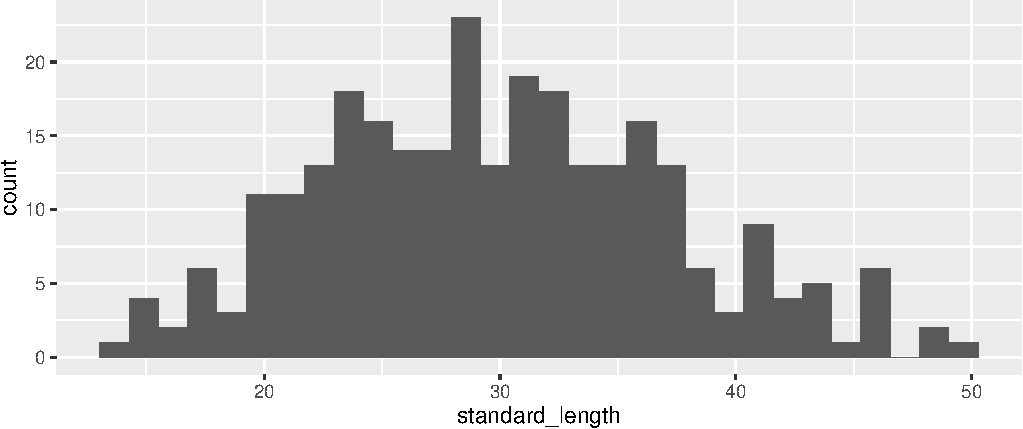
\includegraphics{skeleton_files/figure-latex/unnamed-chunk-20-1.pdf}

Note that \texttt{ggplot} uses the \texttt{+} symbol to \textbf{add}
layers to the plot. This is similar to the piping symbol and it's easy
to get them switched.\\
By default, \texttt{ggplot} specifies a \texttt{binwidth} of
\(range / 30\), where \(range\) corresponds to the largest value in the
data set minus the smallest values in the data set. It also uses black
fill as the default choice. We can tweak the \texttt{binwidth},
\texttt{fill} color, and outline \texttt{colour} by specifying those
arguments inside the \texttt{geom\_histogram} function:

\begin{Shaded}
\begin{Highlighting}[]
\NormalTok{length_data %>%}\StringTok{ }\KeywordTok{ggplot}\NormalTok{(}\KeywordTok{aes}\NormalTok{(}\DataTypeTok{x =} \NormalTok{standard_length)) +}
\StringTok{  }\KeywordTok{geom_histogram}\NormalTok{(}\DataTypeTok{binwidth =} \FloatTok{2.5}\NormalTok{, }\DataTypeTok{fill =} \StringTok{"darkseagreen"}\NormalTok{, }
                 \DataTypeTok{colour =} \StringTok{"black"}\NormalTok{)}
\end{Highlighting}
\end{Shaded}

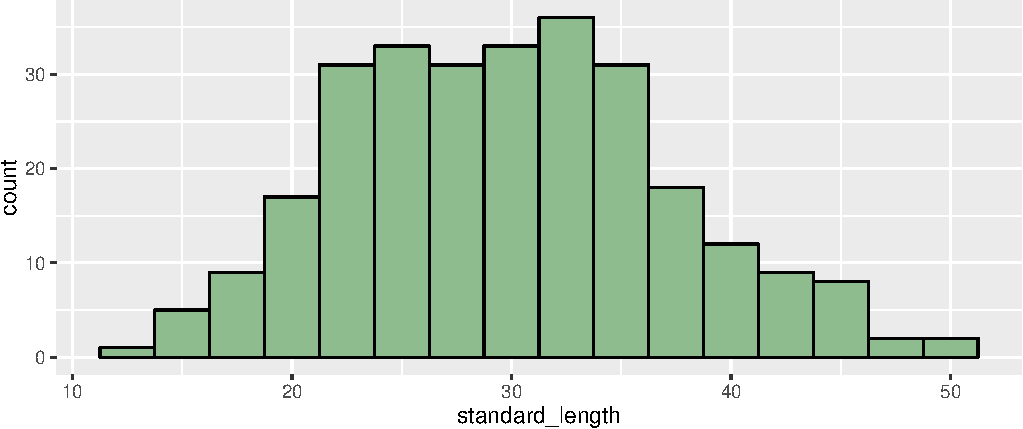
\includegraphics{skeleton_files/figure-latex/unnamed-chunk-21-1.pdf}

\emph{Helpful Note}: A listing of all the built-in colors by name is
available
\href{http://www.stat.columbia.edu/~tzheng/files/Rcolor.pdf}{here}.

In order to test hypotheses, we need to describe frequency distributions
by calculating several statistics. This can be accomplished quite easily
using the \texttt{summarize} function in the \texttt{dplyr} package:

\begin{Shaded}
\begin{Highlighting}[]
\NormalTok{summary_stats <-}\StringTok{ }\NormalTok{length_data %>%}
\StringTok{  }\KeywordTok{summarize}\NormalTok{(}\DataTypeTok{mean =} \KeywordTok{mean}\NormalTok{(standard_length),}
            \DataTypeTok{std_dev =} \KeywordTok{sd}\NormalTok{(standard_length),}
            \DataTypeTok{N =} \KeywordTok{n}\NormalTok{(),}
            \DataTypeTok{std_err =} \NormalTok{std_dev /}\StringTok{ }\KeywordTok{sqrt}\NormalTok{(N),}
            \DataTypeTok{lower_CI_limit =} \NormalTok{mean +}\StringTok{ }\KeywordTok{qt}\NormalTok{(}\FloatTok{0.025}\NormalTok{, }\DataTypeTok{df =} \NormalTok{N -}\StringTok{ }\DecValTok{1}\NormalTok{) *}\StringTok{ }\NormalTok{std_err,}
            \DataTypeTok{upper_CI_limit =} \NormalTok{mean +}\StringTok{ }\KeywordTok{qt}\NormalTok{(}\FloatTok{0.975}\NormalTok{, }\DataTypeTok{df =} \NormalTok{N -}\StringTok{ }\DecValTok{1}\NormalTok{) *}\StringTok{ }\NormalTok{std_err)}
\NormalTok{summary_stats}
\end{Highlighting}
\end{Shaded}

\begin{Verbatim}[frame=single]
Source: local data frame [1 x 6]

      mean  std_dev     N   std_err lower_CI_limit upper_CI_limit
     <dbl>    <dbl> <int>     <dbl>          <dbl>          <dbl>
1 29.87827 7.357723   278 0.4412869       29.00957       30.74698
\end{Verbatim}

As you can see, six calculations have been made here:

\begin{itemize}
\tightlist
\item
  \texttt{mean}: the mean of the \texttt{standard\_length} variable
\item
  \texttt{std\_dev}: the standard deviation of the
  \texttt{standard\_length} variable
\item
  \texttt{N}: the number of observations in the
  \texttt{standard\_length} variable
\item
  \texttt{std\_err}: the standard error of the mean of the
  \texttt{standard\_length} variable
\item
  \texttt{lower\_CI\_limit}: the lower bound of a 95\% confidence
  interval for the corresponding population mean of the
  \texttt{standard\_length} variable
\item
  \texttt{upper\_CI\_limit}: the upper bound of a 95\% confidence
  interval for the corresponding population mean of the
  \texttt{standard\_length} variable
\end{itemize}

\medskip

\textbf{Overlaying a normal distribution}

After you have calculated these summary statistics, you can also use
these \texttt{mean} and \texttt{std\_dev} variables as inputs into the
mean and standard deviation of a normal distribution. You can then plot
this normal distribution over the top of your frequency distribution to
provide a visual as to how well the data could be represented by a
normal curve. The function related to this curve is the \textbf{normal
density curve} which is denoted as \texttt{dnorm} in R:

\begin{Shaded}
\begin{Highlighting}[]
\NormalTok{length_data %>%}\StringTok{ }\KeywordTok{ggplot}\NormalTok{(}\KeywordTok{aes}\NormalTok{(}\DataTypeTok{x =} \NormalTok{standard_length)) +}
\StringTok{  }\KeywordTok{geom_histogram}\NormalTok{(}\KeywordTok{aes}\NormalTok{(}\DataTypeTok{y =} \NormalTok{..density..), }\DataTypeTok{binwidth =} \FloatTok{2.5}\NormalTok{, }
                 \DataTypeTok{fill =} \StringTok{"darkseagreen"}\NormalTok{, }
                 \DataTypeTok{colour =} \StringTok{"black"}\NormalTok{) +}
\StringTok{  }\KeywordTok{stat_function}\NormalTok{(}\DataTypeTok{fun =} \NormalTok{dnorm, }
                \DataTypeTok{args =} \KeywordTok{list}\NormalTok{(}\DataTypeTok{mean =} \NormalTok{summary_stats$mean,}
                            \DataTypeTok{sd =} \NormalTok{summary_stats$std_dev),}
                \DataTypeTok{colour =} \StringTok{"red"}\NormalTok{)}
\end{Highlighting}
\end{Shaded}

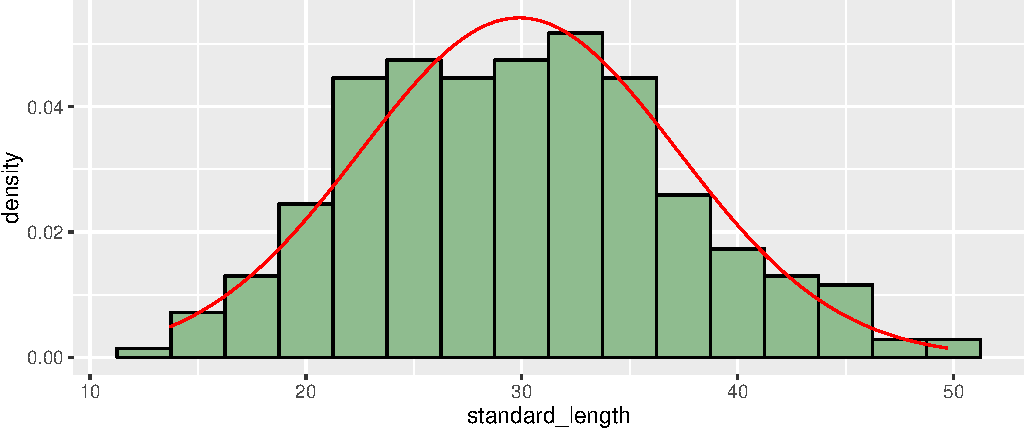
\includegraphics{skeleton_files/figure-latex/unnamed-chunk-23-1.pdf}

Note here the addition of the \texttt{aes(y\ =\ ..density..)} parameter
which puts the normal curve and the histogram on the same scale. Density
corresponds to the percentage of values that fall in a given bin which
is just the transformation of \texttt{count\ /\ N}.

\nonumsection{Producing counts of subsets}

The \texttt{summarize} function you saw earlier can also be used to
produce summaries of subsets of data by using the \texttt{group\_by}
function. A larger collection of data similar to that seen with the
height measurements at a lake/pond on different days of the week is used
to show an example of this. We begin by reading the data into a data
frame:

\begin{Shaded}
\begin{Highlighting}[]
\NormalTok{water_full <-}\StringTok{ }\KeywordTok{read_csv}\NormalTok{(}\StringTok{"data/water_data.csv"}\NormalTok{)}
\end{Highlighting}
\end{Shaded}

Next we will calculate the mean and standard deviation of
\texttt{body\_height} for both levels of \texttt{location}:

\begin{Shaded}
\begin{Highlighting}[]
\NormalTok{location_summaries <-}\StringTok{ }\NormalTok{water_full %>%}\StringTok{ }\KeywordTok{group_by}\NormalTok{(location) %>%}
\StringTok{  }\KeywordTok{summarize}\NormalTok{(}\DataTypeTok{mean =} \KeywordTok{mean}\NormalTok{(body_height),}
            \DataTypeTok{std_dev =} \KeywordTok{sd}\NormalTok{(body_height))}
\NormalTok{location_summaries}
\end{Highlighting}
\end{Shaded}

\begin{Verbatim}[frame=single]
Source: local data frame [2 x 3]

  location      mean  std_dev
     <chr>     <dbl>    <dbl>
1     lake 10.513333 1.467790
2     pond  7.740095 1.308003
\end{Verbatim}

We can further group by \texttt{location} and \texttt{day\_of\_lab} to
get a summary for all combinations of those two variables. Notice how
similar this code is to the chunk immediately above:

\begin{Shaded}
\begin{Highlighting}[]
\NormalTok{location_day_summaries <-}\StringTok{ }\NormalTok{water_full %>%}\StringTok{ }
\StringTok{  }\KeywordTok{group_by}\NormalTok{(day_of_lab, location) %>%}
\StringTok{  }\KeywordTok{summarize}\NormalTok{(}\DataTypeTok{mean =} \KeywordTok{mean}\NormalTok{(body_height),}
            \DataTypeTok{std_dev =} \KeywordTok{sd}\NormalTok{(body_height))}
\NormalTok{location_day_summaries}
\end{Highlighting}
\end{Shaded}

\begin{Verbatim}[frame=single]
Source: local data frame [8 x 4]
Groups: day_of_lab [?]

  day_of_lab location      mean   std_dev
       <chr>    <chr>     <dbl>     <dbl>
1     Friday     lake 10.203000 0.7005244
2     Friday     pond  7.940200 0.9795852
3   Thursday     lake 11.098000 1.0748933
4   Thursday     pond  8.252909 0.8172019
5    Tuesday     lake  8.855556 1.3146683
6    Tuesday     pond  7.640000 1.9488407
7  Wednesday     lake 11.731000 1.0155945
8  Wednesday     pond  7.086000 1.0093804
\end{Verbatim}

\section{\texorpdfstring{Probability (\(P\)) Values and the Null
Hypothesis}{Probability (P) Values and the Null Hypothesis}}\label{probability-p-values-and-the-null-hypothesis}

Statistical tests are devised to test a \textbf{null hypothesis} of no
statistically significant effect of X (treatments) on Y (measured
response variable). They result in a probability (p-value) that these
results could exist by chance.

If the probability is low enough (p \textless{} 0.05), we can reject the
null hypothesis and support the alternate hypothesis that X is
statistically significantly affecting Y.

Write this inside the cover of your lab notebook to refer to when you do
a statistical test:

\textbf{If p is greater than (\textgreater{}) 0.05, then you can't
reject the null hypothesis.}

\textbf{If p is less than (\textless{}) 0.05, then you can reject the
null hypothesis.}

Another way to think about this is:

\begin{quote}
If p \textgreater{} 0.05, there is no statistically significant effect
of X on Y.
\end{quote}

You never \underline{accept} the null hypothesis. You can only
\underline{fail to reject} the null hypothesis.

If p \textless{} 0.05, there is a statistically significant effect of X
on Y.

You never \underline{prove} the hypothesis.

You can only \underline{support} the alternate hypothesis by rejecting
the null hypothesis.

At this point, your job is to describe the \underline{direction}
(positive or negative, \textless{} or \textgreater{}) of the significant
effect.

Depending on the type of test, this could be stated as:

\begin{quote}
As X increases, Y statistically significantly \underline{increases} (or
decreases).
\end{quote}

or

\begin{quote}
X Group A has a statistically significantly \underline{greater} mean Y
than X Group B.
\end{quote}

Remember that statistical significance and biological relevance are not
the same.

See page G-2-3 for more information.

\section{Reporting on Statistical
Results}\label{reporting-on-statistical-results}

Scientific writing is very efficient.

One super-informative sentence can summarize the same information as six
sentences.

\begin{enumerate}
\def\labelenumi{\arabic{enumi}.}
\tightlist
\item
  The mean standard length for stickleback fish in the pond (38.9 mm)
  was statistically significantly greater than in the lake (35.9 mm)
  (ANOVA, F = 12.6, df = 1, 452, p = 0.0004).
\end{enumerate}

instead of

\begin{quote}
\begin{enumerate}
\def\labelenumi{\arabic{enumi}.}
\tightlist
\item
  The null hypothesis is that the mean Y values for treatments A and B
  were not statistically significantly different.
\end{enumerate}
\end{quote}

\begin{quote}
\begin{enumerate}
\def\labelenumi{\arabic{enumi}.}
\setcounter{enumi}{1}
\tightlist
\item
  We can reject the null hypothesis, as the p-value was less than 0.05.
\end{enumerate}
\end{quote}

\begin{quote}
\begin{enumerate}
\def\labelenumi{\arabic{enumi}.}
\setcounter{enumi}{2}
\tightlist
\item
  There is a statistically significant difference.
\end{enumerate}
\end{quote}

\begin{quote}
\begin{enumerate}
\def\labelenumi{\arabic{enumi}.}
\setcounter{enumi}{3}
\tightlist
\item
  The difference is that the mean for A is greater than for B.
\end{enumerate}
\end{quote}

\begin{quote}
\begin{enumerate}
\def\labelenumi{\arabic{enumi}.}
\setcounter{enumi}{4}
\tightlist
\item
  The mean for A was \#, while the mean for B was \#.
\end{enumerate}
\end{quote}

\begin{quote}
\begin{enumerate}
\def\labelenumi{\arabic{enumi}.}
\setcounter{enumi}{5}
\tightlist
\item
  The ANOVA results were that F = \#, the df = \#, \# and the p = \#.
\end{enumerate}
\end{quote}

Using the phrase ``statistically significantly'' implies that the null
hypothesis was rejected based on the p-value being less than 0.05.

Your lab notebook is an appropriate place to write out the six sentences
to keep track of the logic.

In a lab report, the null hypothesis being tested should be mentioned
near the end of the Materials and Methods section, and the single
summary sentence should be used in the Results section.

\section{Analysis of Variance (ANOVA)}\label{analysis-of-variance-anova}

\subsection*{Univariate, single factor, one-way
ANOVA}\label{univariate-single-factor-one-way-anova}
\addcontentsline{toc}{subsection}{Univariate, single factor, one-way
ANOVA}

An appropriate data set for this type of analysis includes one column
containing nominal \texttt{chr} data that represents the different (more
than 2) treatments and one column containing continuous \texttt{int} or
\texttt{dbl} data that represent the measured responses to the
treatments. An example is below:

\begin{Shaded}
\begin{Highlighting}[]
\NormalTok{day_of_lab <-}\StringTok{ }\KeywordTok{c}\NormalTok{(}\KeywordTok{rep}\NormalTok{(}\StringTok{"Tuesday"}\NormalTok{, }\DecValTok{5}\NormalTok{), }\KeywordTok{rep}\NormalTok{(}\StringTok{"Wednesday"}\NormalTok{, }\DecValTok{5}\NormalTok{), }
                \KeywordTok{rep}\NormalTok{(}\StringTok{"Thursday"}\NormalTok{, }\DecValTok{5}\NormalTok{))}
\NormalTok{standard_length <-}\StringTok{ }\KeywordTok{c}\NormalTok{(}\FloatTok{38.4}\NormalTok{, }\FloatTok{46.2}\NormalTok{, }\FloatTok{32.2}\NormalTok{, }\FloatTok{35.7}\NormalTok{, }\FloatTok{39.4}\NormalTok{, }
                     \DecValTok{28}\NormalTok{, }\FloatTok{31.8}\NormalTok{, }\DecValTok{35}\NormalTok{, }\FloatTok{29.3}\NormalTok{, }\FloatTok{30.1}\NormalTok{,}
                     \FloatTok{33.33}\NormalTok{, }\FloatTok{33.23}\NormalTok{, }\FloatTok{35.2}\NormalTok{, }\FloatTok{35.99}\NormalTok{, }\FloatTok{30.81}\NormalTok{)}
\NormalTok{anova_data <-}\StringTok{ }\KeywordTok{data_frame}\NormalTok{(day_of_lab, standard_length)}
\NormalTok{anova_data}
\end{Highlighting}
\end{Shaded}

\begin{Verbatim}[frame=single]
Source: local data frame [15 x 2]

   day_of_lab standard_length
        <chr>           <dbl>
1     Tuesday           38.40
2     Tuesday           46.20
3     Tuesday           32.20
4     Tuesday           35.70
5     Tuesday           39.40
6   Wednesday           28.00
7   Wednesday           31.80
8   Wednesday           35.00
9   Wednesday           29.30
10  Wednesday           30.10
11   Thursday           33.33
12   Thursday           33.23
13   Thursday           35.20
14   Thursday           35.99
15   Thursday           30.81
\end{Verbatim}

The \texttt{aov()} function fits an Analysis of Variance model with at
least one predictor variable and a response variable. Here the response
is \texttt{standard\_length} and the predictor is \texttt{day\_of\_lab}.
In other words, we are looking to see if there is statistical evidence
that at least one difference exists in mean \texttt{standard\_length}
for Tuesday, Wednesday, and Thursday. The variable
\texttt{length\_model} is defined to store the resulting values obtained
by the ANOVA fit. The \texttt{anova()} function is then used on
\texttt{length\_model} to produce the corresponding Analysis of Variance
table.

\begin{Shaded}
\begin{Highlighting}[]
\NormalTok{length_model <-}\StringTok{  }\KeywordTok{aov}\NormalTok{(standard_length ~}\StringTok{ }\NormalTok{day_of_lab, }\DataTypeTok{data =} \NormalTok{anova_data)}
\KeywordTok{anova}\NormalTok{(length_model)}
\end{Highlighting}
\end{Shaded}

\begin{Verbatim}[frame=single]
Analysis of Variance Table

Response: standard_length
           Df Sum Sq Mean Sq F value  Pr(>F)  
day_of_lab  2 144.82  72.409  5.6797 0.01838 *
Residuals  12 152.98  12.749                  
---
Signif. codes:  0 '***' 0.001 '**' 0.01 '*' 0.05 '.' 0.1 ' ' 1
\end{Verbatim}

Here, \texttt{F\ value} is the value of the F statistic associated with
the \textbf{ANOVA}. \texttt{Pr\ (\textgreater{}F)} is the
\textbf{p-value}.

A visual representation of this analysis can be achieved by first
calculating summary statistics as before. Here, the columns for count
and standard deviation are omitted.

\begin{Shaded}
\begin{Highlighting}[]
\NormalTok{day_summaries <-}\StringTok{ }\NormalTok{anova_data %>%}\StringTok{ }
\StringTok{  }\KeywordTok{group_by}\NormalTok{(day_of_lab) %>%}
\StringTok{  }\KeywordTok{summarize}\NormalTok{(}\DataTypeTok{mean =} \KeywordTok{mean}\NormalTok{(standard_length),}
            \DataTypeTok{std_dev =} \KeywordTok{sd}\NormalTok{(standard_length),}
            \DataTypeTok{N =} \KeywordTok{n}\NormalTok{(),}
            \DataTypeTok{std_err =} \NormalTok{std_dev /}\StringTok{ }\KeywordTok{sqrt}\NormalTok{(N),}
            \DataTypeTok{lower_CI_limit =} \NormalTok{mean +}\StringTok{ }\KeywordTok{qt}\NormalTok{(}\FloatTok{0.025}\NormalTok{, }\DataTypeTok{df =} \NormalTok{N}\DecValTok{-1}\NormalTok{) *}\StringTok{ }\NormalTok{std_err,}
            \DataTypeTok{upper_CI_limit =} \NormalTok{mean +}\StringTok{ }\KeywordTok{qt}\NormalTok{(}\FloatTok{0.975}\NormalTok{, }\DataTypeTok{df =} \NormalTok{N}\DecValTok{-1}\NormalTok{) *}\StringTok{ }\NormalTok{std_err) %>%}
\StringTok{  }\NormalTok{dplyr::}\KeywordTok{select}\NormalTok{(-N, -std_dev)}
\NormalTok{day_summaries}
\end{Highlighting}
\end{Shaded}

\begin{Verbatim}[frame=single]
Source: local data frame [3 x 5]

  day_of_lab   mean   std_err lower_CI_limit upper_CI_limit
       <chr>  <dbl>     <dbl>          <dbl>          <dbl>
1   Thursday 33.712 0.9000911       31.21295       36.21105
2    Tuesday 38.380 2.3191378       31.94104       44.81896
3  Wednesday 30.840 1.2085529       27.48452       34.19548
\end{Verbatim}

Before plotting, the data frame is sorted to follow the more natural
weekly progression instead of alphabetical order.

\begin{Shaded}
\begin{Highlighting}[]
\NormalTok{reorder <-}\StringTok{ }\KeywordTok{c}\NormalTok{(}\StringTok{"Tuesday"}\NormalTok{, }\StringTok{"Wednesday"}\NormalTok{, }\StringTok{"Thursday"}\NormalTok{)}
\NormalTok{day_summaries %>%}\StringTok{ }
\StringTok{  }\KeywordTok{mutate}\NormalTok{(}\DataTypeTok{day_of_lab =} \KeywordTok{ordered}\NormalTok{(day_of_lab, }\DataTypeTok{levels =} \NormalTok{reorder)) %>%}
\StringTok{  }\KeywordTok{ggplot}\NormalTok{(}\KeywordTok{aes}\NormalTok{(}\DataTypeTok{x =} \NormalTok{day_of_lab, }\DataTypeTok{y =} \NormalTok{mean)) +}
\StringTok{  }\KeywordTok{geom_errorbar}\NormalTok{(}\KeywordTok{aes}\NormalTok{(}\DataTypeTok{ymin =} \NormalTok{lower_CI_limit, }\DataTypeTok{ymax =} \NormalTok{upper_CI_limit), }
                \DataTypeTok{width =} \FloatTok{0.1}\NormalTok{) +}
\StringTok{  }\KeywordTok{geom_point}\NormalTok{(}\DataTypeTok{colour =} \StringTok{"red"}\NormalTok{) +}
\StringTok{  }\KeywordTok{xlab}\NormalTok{(}\StringTok{"Day of Lab"}\NormalTok{) +}
\StringTok{  }\KeywordTok{ylab}\NormalTok{(}\StringTok{"Standard Length (mm)"}\NormalTok{)}
\end{Highlighting}
\end{Shaded}

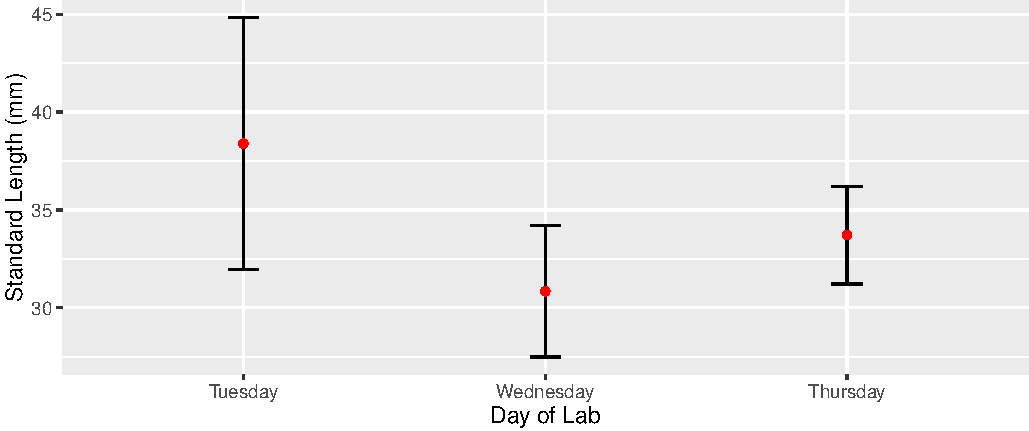
\includegraphics{skeleton_files/figure-latex/unnamed-chunk-30-1.pdf}

\begin{itemize}
\item
  The error bars around the means are the 95\% confidence intervals
  (95\% CI).
\item
  When reporting statistical test results in text, state the result and
  then the supporting test details in parentheses.
\end{itemize}

Summary statement:

The mean stickleback standard length was statistically significantly
greater on Tuesday (38.4 mm) than on Wednesday (30.8 mm) (ANOVA, F =
8.3, df = 1,8, P = 0.02).

\begin{itemize}
\item
  Note that there are two degrees of freedom (df) reported: Model DF and
  Error DF from the Analysis of Variance table.
\item
  The Model DF is based on the number of categories in your X factor -1.
  In the above example, there are 2 days of lab -1 = 1 df.
\item
  The Error DF is based on the Total DF - the Model DF. In the above
  example, Total DF is 9 - 1 = 8 df.
\item
  Sample size N = Total DF + 1.
\end{itemize}

See pages I-5-7 for an explanation of ANOVA.

\section{Post-hoc Tests}\label{post-hoc-tests}

An appropriate data set for this type of analysis includes one column
containing nominal \texttt{chr} data that represents the different (more
than 2) treatments and one column containing continuous \texttt{int} or
\texttt{dbl} data that represent the measured responses to the
treatments.

\begin{itemize}
\item
  If you cannot reject your null hypothesis (ANOVA p\textgreater{}0.05),
  then your analysis is complete.
\item
  If you can reject your null hypothesis (ANOVA p\textless{}0.05), and
  there are three or more groups that are being compared, you might want
  to ask which groups are statistically significantly different from
  each other and which are not statistically significantly different. In
  order to do this, we have to compute \textbf{a posteriori} (after the
  fact) \textbf{p-values}. These are called \textbf{post-hoc tests}.
  There are many ways to do this, but we will suggest a conservative
  method here known as Tukey's Honest Significant Difference.
  \texttt{TukeyHSD} expects an \texttt{aov} fitted model as its
  parameter as we have with \texttt{length\_model}.
\end{itemize}

\begin{Shaded}
\begin{Highlighting}[]
\KeywordTok{TukeyHSD}\NormalTok{(length_model)}
\end{Highlighting}
\end{Shaded}

\begin{Verbatim}[frame=single]
  Tukey multiple comparisons of means
    95% family-wise confidence level

Fit: aov(formula = standard_length ~ day_of_lab, data = anova_data)

$day_of_lab
                     diff        lwr       upr     p adj
Tuesday-Thursday    4.668  -1.356555 10.692555 0.1387553
Wednesday-Thursday -2.872  -8.896555  3.152555 0.4365799
Wednesday-Tuesday  -7.540 -13.564555 -1.515445 0.0150869
\end{Verbatim}

In this one-way \textbf{ANOVA}, there are 3 levels or groups: Tuesday,
Wednesday and Thursday. An ANOVA had already told us that the null
hypothesis could be rejected (p=0.02). Now we are asking if Tuesday's
mean is statistically significantly different than Thursday's mean, and
the answer at the p \textless{} 0.05 level is: no, it is not. The
p-value for that comparison is 0.1387. Is Tuesday's mean statistically
significantly different from Wednesday's mean? Yes, it is. The p-value
for that comparison is 0.01509. Is Thursday's mean statistically
significantly different from Wednesday's mean? No, it is not. The
p-value for that comparison is 0.4366.

Summary statement:

\begin{quote}
Tuesday's mean standard length (38.4 mm) is statistically significantly
greater than Wednesday's mean (30.8 mm), and Thursday's mean (33.7 mm)
is not statistically significantly different from either of the other
groups' means (ANOVA, F = 5.7, df = 2,12, p = 0.02, Tukey post-hoc HSD).
\end{quote}

Using a different post-hoc test such as \textbf{Pairwise t test} will
give similar results. See page I-7 for more explanation.

\section{Bivariate Linear Regression
Analysis}\label{bivariate-linear-regression-analysis}

An appropriate data set for this type of analysis includes two columns
containing continuous \texttt{int} or \texttt{dbl} data that are
associated with each other row by row. An example looking at the
relationship between body height and standard length follows. First, the
data is loaded in.

\begin{Shaded}
\begin{Highlighting}[]
\NormalTok{std_length <-}\StringTok{ }\KeywordTok{c}\NormalTok{(}\DecValTok{22}\NormalTok{, }\FloatTok{23.8}\NormalTok{, }\FloatTok{25.1}\NormalTok{, }\FloatTok{26.9}\NormalTok{, }\DecValTok{27}\NormalTok{, }
                \FloatTok{27.1}\NormalTok{, }\FloatTok{28.7}\NormalTok{, }\FloatTok{29.7}\NormalTok{, }\FloatTok{30.9}\NormalTok{, }\FloatTok{31.5}\NormalTok{, }
                \FloatTok{32.6}\NormalTok{, }\FloatTok{33.8}\NormalTok{, }\FloatTok{34.1}\NormalTok{, }\FloatTok{35.2}\NormalTok{, }\FloatTok{36.2}\NormalTok{)}
\NormalTok{height <-}\StringTok{ }\KeywordTok{c}\NormalTok{(}\FloatTok{5.17}\NormalTok{, }\FloatTok{6.3}\NormalTok{, }\FloatTok{8.5}\NormalTok{, }\FloatTok{7.7}\NormalTok{, }\FloatTok{6.19}\NormalTok{, }
            \FloatTok{7.21}\NormalTok{, }\FloatTok{6.63}\NormalTok{, }\FloatTok{8.54}\NormalTok{, }\FloatTok{8.6}\NormalTok{, }\FloatTok{7.7}\NormalTok{, }
            \FloatTok{7.8}\NormalTok{, }\FloatTok{9.79}\NormalTok{, }\FloatTok{8.64}\NormalTok{, }\FloatTok{8.8}\NormalTok{, }\FloatTok{8.77}\NormalTok{)}
\NormalTok{reg_example <-}\StringTok{ }\KeywordTok{data_frame}\NormalTok{(std_length, height)}
\end{Highlighting}
\end{Shaded}

Now, a model is fit using the \texttt{lm} function which stands for
``linear model''. Note the order in which the variables are inputted
before and after the ``tilde''.

\begin{Shaded}
\begin{Highlighting}[]
\NormalTok{reg_model <-}\StringTok{ }\KeywordTok{lm}\NormalTok{(height ~}\StringTok{ }\NormalTok{std_length, }\DataTypeTok{data =} \NormalTok{reg_example)}
\end{Highlighting}
\end{Shaded}

We can get a multitude of information about this fit by using the
\texttt{anova()} and \texttt{summary()} functions on
\texttt{reg\_model}:

\begin{Shaded}
\begin{Highlighting}[]
\KeywordTok{anova}\NormalTok{(reg_model)}
\end{Highlighting}
\end{Shaded}

\begin{Verbatim}[frame=single]
Analysis of Variance Table

Response: height
           Df Sum Sq Mean Sq F value    Pr(>F)    
std_length  1 12.773 12.7732  18.495 0.0008623 ***
Residuals  13  8.978  0.6906                      
---
Signif. codes:  0 '***' 0.001 '**' 0.01 '*' 0.05 '.' 0.1 ' ' 1
\end{Verbatim}

\begin{Shaded}
\begin{Highlighting}[]
\KeywordTok{summary}\NormalTok{(reg_model)}
\end{Highlighting}
\end{Shaded}

\begin{Verbatim}[frame=single]

Call:
lm(formula = height ~ std_length, data = reg_example)

Residuals:
    Min      1Q  Median      3Q     Max 
-0.9807 -0.5403 -0.1612  0.5581  1.7506 

Coefficients:
            Estimate Std. Error t value Pr(>|t|)    
(Intercept)  1.18455    1.54301   0.768 0.456393    
std_length   0.22171    0.05155   4.301 0.000862 ***
---
Signif. codes:  0 '***' 0.001 '**' 0.01 '*' 0.05 '.' 0.1 ' ' 1

Residual standard error: 0.831 on 13 degrees of freedom
Multiple R-squared:  0.5872,    Adjusted R-squared:  0.5555 
F-statistic:  18.5 on 1 and 13 DF,  p-value: 0.0008623
\end{Verbatim}

\begin{itemize}
\tightlist
\item
  The equation for the straight line \(\hat{Y} = b + mX\) corresponding
  to the fit is taken from the \texttt{Coefficients:} table:
\end{itemize}

\[ \hat{Body \text{ } Height \text{ } (mm)} = 1.18455 + 0.22171 * [Standard \text{ } Length \text{ } (mm)] \]

\begin{itemize}
\item
  \texttt{F\ value} is the F statistic associated with \textbf{ANOVA}.
\item
  \texttt{Pr\ (\textgreater{}F)} is the corresponding \textbf{p-value}.
\item
  When reporting statistical test results in text, state the result and
  then the supporting test details in parentheses.
\end{itemize}

Summary statement:

\begin{quote}
There is a statistically significant positive relationship between
standard length and body height in stickleback fish (ANOVA, F = 18.5, df
= 1,13, p = 0.0008).
\end{quote}

\begin{itemize}
\item
  Note that there are two degrees of freedom (df) reported. The first is
  the Model DF and the second is the Error DF from the Analysis of
  Variance table (\texttt{Residuals}).
\item
  Sample size N= Total DF + 1.
\item
  \textbf{Multiple R-squared} varies from 0 (no fit) to 1 (perfect fit
  of all points to the line).
\end{itemize}

See page I-8 for more explanation.

A plot showing the relationship between the two variables follows. Also
on the plot is the best-fit line through your data points and the 95\%
confidence intervals for the true slope.

\begin{Shaded}
\begin{Highlighting}[]
\NormalTok{reg_example %>%}\StringTok{ }\KeywordTok{ggplot}\NormalTok{(}\KeywordTok{aes}\NormalTok{(}\DataTypeTok{x =} \NormalTok{std_length, }\DataTypeTok{y =} \NormalTok{height)) +}
\StringTok{  }\KeywordTok{geom_point}\NormalTok{() +}
\StringTok{  }\KeywordTok{geom_smooth}\NormalTok{(}\DataTypeTok{method =} \NormalTok{lm, }\DataTypeTok{se =} \OtherTok{TRUE}\NormalTok{)}
\end{Highlighting}
\end{Shaded}

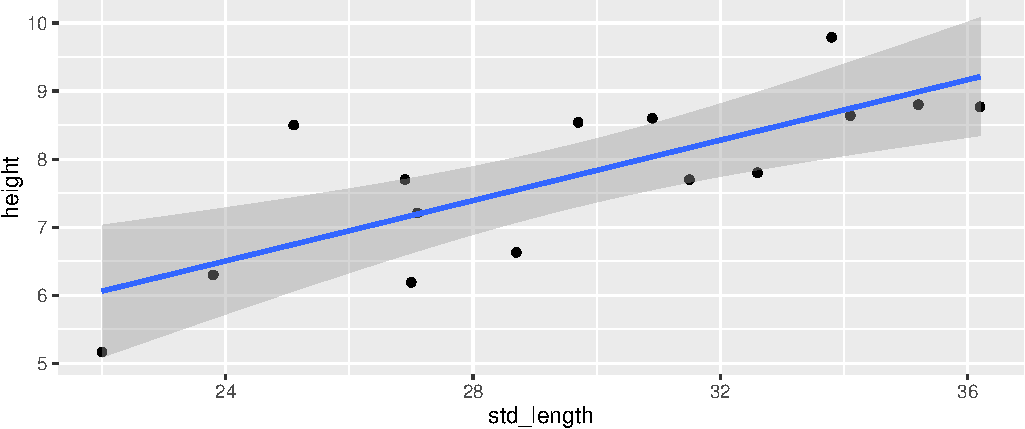
\includegraphics{skeleton_files/figure-latex/unnamed-chunk-35-1.pdf}

\section{ANCOVA}\label{ancova}

An appropriate data set includes one column containing nominal
\texttt{chr} data that represents the different (more than 2) treatments
and two columns containing continuous \texttt{int} or \texttt{dbl} data
that represent the measured responses to the treatments.

\begin{Shaded}
\begin{Highlighting}[]
\NormalTok{ancova_example <-}\StringTok{ }\KeywordTok{read_csv}\NormalTok{(}\StringTok{"data/ANCOVA.csv"}\NormalTok{)}
\end{Highlighting}
\end{Shaded}

Here, \texttt{Body\ Height\ (mm)} will be Y variable status (also called
response variable, dependent variable, and is the variable you actually
measured.) There are two explanatory X variables: the continuous
\texttt{Standard\ Length\ (mm)} and the nominal \texttt{Location}.
Finally, and most importantly, to finish adding the X factors, you must
allow for an \textbf{interaction} term. This essentially tests whether
the effects of any X variable on Y is dependent on other X variables in
the model. Notice the full interaction model in the code below.

\begin{Shaded}
\begin{Highlighting}[]
\NormalTok{ancova_model <-}\StringTok{ }\KeywordTok{aov}\NormalTok{(Body_Height_mm ~}\StringTok{ }\NormalTok{Standard_Length_mm +}\StringTok{ }\NormalTok{Location }
                    \NormalTok{+}\StringTok{ }\NormalTok{Standard_Length_mm:Location, }
                    \DataTypeTok{data =} \NormalTok{ancova_example)}
\KeywordTok{anova}\NormalTok{(ancova_model)}
\end{Highlighting}
\end{Shaded}

\begin{Verbatim}[frame=single]
Analysis of Variance Table

Response: Body_Height_mm
                            Df Sum Sq Mean Sq F value  Pr(>F)   
Standard_Length_mm           1 3.2505  3.2505 27.1180 0.00200 **
Location                     1 0.0021  0.0021  0.0179 0.89796   
Standard_Length_mm:Location  1 0.8892  0.8892  7.4184 0.03447 * 
Residuals                    6 0.7192  0.1199                   
---
Signif. codes:  0 '***' 0.001 '**' 0.01 '*' 0.05 '.' 0.1 ' ' 1
\end{Verbatim}

Notice the p-values (\texttt{Pr(\textgreater{}F)}) for each of the terms
you are testing in the Analysis of Variance Table.

Summary statements:

\begin{quote}
There is a statistically significant positive relationship between
standard length and body height (ANCOVA, F = 27.1180, df = 1,6, P =
0.002).
\end{quote}

\begin{quote}
There is no statistically significant difference between lake and pond
in the height of the regression lines for standard length vs.~body
height (ANCOVA, F = 0.0179, df = 1,6, P = 0.89796).
\end{quote}

\begin{quote}
There is a statistically significantly steeper slope for lake than pond
for the relationship between standard length and body height (ANCOVA, F
= 7.4184, df = 1,6 , P = 0.03447).
\end{quote}

\begin{itemize}
\item
  There are two degrees of freedom (df) reported. The first is the DF
  for each effect in the Analysis of Variance table, and the second is
  the Error DF from the Analysis of Variance table (\texttt{Residuals}).
\item
  Sample size N= Total DF + 1.
\end{itemize}

See page I-9 for more explanation.

A plot showing the relationship between \texttt{Standard\_Length\_mm}
and \texttt{Body\_Height\_mm} as well as the best-fit line through your
data points for both \texttt{lake} and \texttt{pond} values follows.
Notice that the points are colored corresponding to which
\texttt{Location} they were measured.

\begin{Shaded}
\begin{Highlighting}[]
\NormalTok{ancova_example %>%}\StringTok{ }\KeywordTok{ggplot}\NormalTok{(}\KeywordTok{aes}\NormalTok{(}\DataTypeTok{x =} \NormalTok{Standard_Length_mm, }
                              \DataTypeTok{y =} \NormalTok{Body_Height_mm, }
                              \DataTypeTok{colour =} \NormalTok{Location)) +}
\StringTok{  }\KeywordTok{geom_point}\NormalTok{() +}
\StringTok{  }\KeywordTok{geom_smooth}\NormalTok{(}\DataTypeTok{method =} \NormalTok{lm, }\DataTypeTok{se =} \OtherTok{FALSE}\NormalTok{)}
\end{Highlighting}
\end{Shaded}

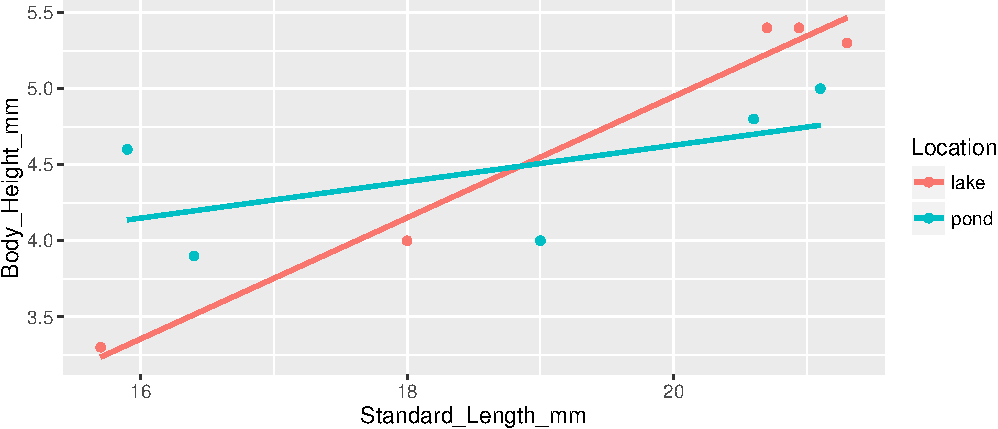
\includegraphics{skeleton_files/figure-latex/unnamed-chunk-38-1.pdf}

\section{Two-Way ANOVA}\label{two-way-anova}

An appropriate data set for this type of analysis includes two columns
containing nominal \texttt{chr} data that represents the different (more
than 2) treatments and one column containing continuous \texttt{int} or
\texttt{dbl} data that represent the measured responses to the
treatments. An example is below:

\begin{Shaded}
\begin{Highlighting}[]
\NormalTok{two_way_anova_example <-}\StringTok{ }\KeywordTok{read_csv}\NormalTok{(}\StringTok{"data/two_way_ANOVA.csv"}\NormalTok{)}
\end{Highlighting}
\end{Shaded}

Here, \texttt{Standard\ Length\ (mm)} will be Y variable status (also
called response variable, dependent variable, and is the variable you
actually measured.) There are two explanatory X variables: the nominal
\texttt{Day\ of\ Lab} and the nominal \texttt{Location}. Finally, and
most importantly, to finish adding the X factors, you must allow for an
\textbf{interaction} term. This essentially tests whether the effects of
any X variable on Y is dependent on other X variables in the model.
Notice the full interaction model in the code below. (Note that you can
only specify the interaction using \texttt{*} and it will by default add
back in the non-interaction terms.)

\begin{Shaded}
\begin{Highlighting}[]
\NormalTok{two_way_model <-}\StringTok{ }\KeywordTok{aov}\NormalTok{(Standard_Length_mm ~}\StringTok{ }\NormalTok{Day_of_Lab *}\StringTok{ }\NormalTok{Location,}
                    \DataTypeTok{data =} \NormalTok{two_way_anova_example)}
\KeywordTok{anova}\NormalTok{(two_way_model)}
\end{Highlighting}
\end{Shaded}

\begin{Verbatim}[frame=single]
Analysis of Variance Table

Response: Standard_Length_mm
                    Df Sum Sq Mean Sq F value    Pr(>F)    
Day_of_Lab           1  997.0   997.0  6.5158   0.01508 *  
Location             1 8979.0  8979.0 58.6816 4.556e-09 ***
Day_of_Lab:Location  1  805.5   805.5  5.2643   0.02771 *  
Residuals           36 5508.4   153.0                      
---
Signif. codes:  0 '***' 0.001 '**' 0.01 '*' 0.05 '.' 0.1 ' ' 1
\end{Verbatim}

Notice the p-values (\texttt{Pr(\textgreater{}F)}) for each of the terms
you are testing in the Analysis of Variance Table. A further breakdown
of means, standard errors, and confidence intervals for different
groupings is below.

\begin{Shaded}
\begin{Highlighting}[]
\NormalTok{location_summaries <-}\StringTok{ }\NormalTok{two_way_anova_example %>%}\StringTok{ }
\StringTok{  }\KeywordTok{group_by}\NormalTok{(Location) %>%}
\StringTok{  }\KeywordTok{summarize}\NormalTok{(}\DataTypeTok{mean =} \KeywordTok{mean}\NormalTok{(Standard_Length_mm),}
            \DataTypeTok{std_dev =} \KeywordTok{sd}\NormalTok{(Standard_Length_mm),}
            \DataTypeTok{N =} \KeywordTok{n}\NormalTok{(),}
            \DataTypeTok{std_err =} \NormalTok{std_dev /}\StringTok{ }\KeywordTok{sqrt}\NormalTok{(N)) %>%}
\StringTok{  }\NormalTok{dplyr::}\KeywordTok{select}\NormalTok{(-N, -std_dev)}
\NormalTok{location_summaries}
\end{Highlighting}
\end{Shaded}

\begin{Verbatim}[frame=single]
Source: local data frame [2 x 3]

  Location   mean  std_err
     <chr>  <dbl>    <dbl>
1     Lake 58.590 3.420964
2     Pond 28.625 2.745243
\end{Verbatim}

\begin{Shaded}
\begin{Highlighting}[]
\NormalTok{day_lab_summaries <-}\StringTok{ }\NormalTok{two_way_anova_example %>%}\StringTok{ }
\StringTok{  }\KeywordTok{group_by}\NormalTok{(Day_of_Lab) %>%}
\StringTok{  }\KeywordTok{summarize}\NormalTok{(}\DataTypeTok{mean =} \KeywordTok{mean}\NormalTok{(Standard_Length_mm),}
            \DataTypeTok{std_dev =} \KeywordTok{sd}\NormalTok{(Standard_Length_mm),}
            \DataTypeTok{N =} \KeywordTok{n}\NormalTok{(),}
            \DataTypeTok{std_err =} \NormalTok{std_dev /}\StringTok{ }\KeywordTok{sqrt}\NormalTok{(N),}
            \DataTypeTok{lower_CI_limit =} \NormalTok{mean +}\StringTok{ }\KeywordTok{qt}\NormalTok{(}\FloatTok{0.025}\NormalTok{, }\DataTypeTok{df =} \NormalTok{N}\DecValTok{-1}\NormalTok{) *}\StringTok{ }\NormalTok{std_err,}
            \DataTypeTok{upper_CI_limit =} \NormalTok{mean +}\StringTok{ }\KeywordTok{qt}\NormalTok{(}\FloatTok{0.975}\NormalTok{, }\DataTypeTok{df =} \NormalTok{N}\DecValTok{-1}\NormalTok{) *}\StringTok{ }\NormalTok{std_err) %>%}
\StringTok{  }\NormalTok{dplyr::}\KeywordTok{select}\NormalTok{(-N, -std_dev)}
\NormalTok{day_lab_summaries}
\end{Highlighting}
\end{Shaded}

\begin{Verbatim}[frame=single]
Source: local data frame [2 x 5]

  Day_of_Lab   mean  std_err lower_CI_limit upper_CI_limit
       <chr>  <dbl>    <dbl>          <dbl>          <dbl>
1    Tuesday 48.600 5.291995       37.52373       59.67627
2  Wednesday 38.615 3.498490       31.29258       45.93742
\end{Verbatim}

\begin{Shaded}
\begin{Highlighting}[]
\NormalTok{day_loc_summaries <-}\StringTok{ }\NormalTok{two_way_anova_example %>%}\StringTok{ }
\StringTok{  }\KeywordTok{group_by}\NormalTok{(Day_of_Lab, Location) %>%}
\StringTok{  }\KeywordTok{summarize}\NormalTok{(}\DataTypeTok{mean =} \KeywordTok{mean}\NormalTok{(Standard_Length_mm),}
            \DataTypeTok{std_dev =} \KeywordTok{sd}\NormalTok{(Standard_Length_mm),}
            \DataTypeTok{N =} \KeywordTok{n}\NormalTok{(),}
            \DataTypeTok{std_err =} \NormalTok{std_dev /}\StringTok{ }\KeywordTok{sqrt}\NormalTok{(N),}
            \DataTypeTok{lower_CI_limit =} \NormalTok{mean +}\StringTok{ }\KeywordTok{qt}\NormalTok{(}\FloatTok{0.025}\NormalTok{, }\DataTypeTok{df =} \NormalTok{N}\DecValTok{-1}\NormalTok{) *}\StringTok{ }\NormalTok{std_err,}
            \DataTypeTok{upper_CI_limit =} \NormalTok{mean +}\StringTok{ }\KeywordTok{qt}\NormalTok{(}\FloatTok{0.975}\NormalTok{, }\DataTypeTok{df =} \NormalTok{N}\DecValTok{-1}\NormalTok{) *}\StringTok{ }\NormalTok{std_err) %>%}
\StringTok{  }\NormalTok{dplyr::}\KeywordTok{select}\NormalTok{(-N, -std_dev)}
\NormalTok{day_loc_summaries}
\end{Highlighting}
\end{Shaded}

\begin{Verbatim}[frame=single]
Source: local data frame [4 x 6]
Groups: Day_of_Lab [2]

  Day_of_Lab Location  mean  std_err lower_CI_limit upper_CI_limit
       <chr>    <chr> <dbl>    <dbl>          <dbl>          <dbl>
1    Tuesday     Lake 68.07 4.418447       58.07478       78.06522
2    Tuesday     Pond 29.13 3.805436       20.52151       37.73849
3  Wednesday     Lake 49.11 3.149407       41.98555       56.23445
4  Wednesday     Pond 28.12 4.157184       18.71580       37.52420
\end{Verbatim}

Lastly, for tests with P\textless{}0.05 and three or more groups, you
can examine Tukey's Honest Significant Difference. The \texttt{\$} and
code following it here corresponds to focusing on the interaction terms
(the only variable with more than two groups).

\begin{Shaded}
\begin{Highlighting}[]
\KeywordTok{TukeyHSD}\NormalTok{(two_way_model)$}\StringTok{`}\DataTypeTok{Day_of_Lab:Location}\StringTok{`}
\end{Highlighting}
\end{Shaded}

\begin{Verbatim}[frame=single]
                                diff      lwr        upr        p adj
Wednesday:Lake-Tuesday:Lake   -18.96 -33.8588  -4.061199 8.023893e-03
Tuesday:Pond-Tuesday:Lake     -38.94 -53.8388 -24.041199 1.716766e-07
Wednesday:Pond-Tuesday:Lake   -39.95 -54.8488 -25.051199 9.923381e-08
Tuesday:Pond-Wednesday:Lake   -19.98 -34.8788  -5.081199 4.876671e-03
Wednesday:Pond-Wednesday:Lake -20.99 -35.8888  -6.091199 2.943201e-03
Wednesday:Pond-Tuesday:Pond    -1.01 -15.9088  13.888801 9.977989e-01
\end{Verbatim}

Summary statements:

\begin{quote}
The mean stickleback standard length was statistically significantly
larger in the lake (58.6 mm) than the pond (28.6 mm) (Two way ANOVA, F =
58.7, df = 1,36, p \textless{} 0.0001).
\end{quote}

\begin{quote}
The mean stickleback standard length was statistically significantly
larger on Tuesday (48.6 mm) than on Wednesday (38.6 mm) (Two way ANOVA,
F = 6.5, df = 1,36, p = 0.02).
\end{quote}

\begin{quote}
There is a statistically significant interaction effect in that in the
lake, the mean standard length for Tuesday (68.1 mm) was statistically
significantly larger than for Wednesday (49.1 mm), but in the pond, the
Tuesday (29.1 mm) and Wednesday (28.1 mm) means were not statistically
significantly different (Two way ANOVA, F = 5.3, df = 1, 36, p =
0.02771, Tukey post-hoc HSD).
\end{quote}

\begin{itemize}
\item
  There are two degrees of freedom (df) reported. The first is the DF
  for each effect in the Effect Tests table, and the second is the Error
  DF from the Analysis of Variance table (\texttt{Residuals}).
\item
  Sample size N= Total DF + 1.
\item
  See the next discussion for the appropriate graph showing the means
  and 95\% CI for each of the subgroups.
\end{itemize}

See page H-20 for post-hoc test interpretation.

See page I-10 for more explanation.

\newpage

To visualize the summaries given above, we can make plots that include
error bars. We can plot the same data with different order of X
Categories.

\begin{Shaded}
\begin{Highlighting}[]
\NormalTok{dodge <-}\StringTok{ }\KeywordTok{position_dodge}\NormalTok{(}\DataTypeTok{width =} \FloatTok{0.1}\NormalTok{)}
\NormalTok{day_loc_summaries %>%}\StringTok{ }
\StringTok{  }\KeywordTok{ggplot}\NormalTok{(}\KeywordTok{aes}\NormalTok{(}\DataTypeTok{x =} \NormalTok{Day_of_Lab, }\DataTypeTok{y =} \NormalTok{mean, }\DataTypeTok{colour =} \NormalTok{Location)) +}
\StringTok{  }\KeywordTok{geom_errorbar}\NormalTok{(}\KeywordTok{aes}\NormalTok{(}\DataTypeTok{ymin =} \NormalTok{lower_CI_limit, }\DataTypeTok{ymax =} \NormalTok{upper_CI_limit), }
                \DataTypeTok{width =} \FloatTok{0.1}\NormalTok{, }\DataTypeTok{position =} \NormalTok{dodge) +}
\StringTok{  }\KeywordTok{geom_point}\NormalTok{(}\DataTypeTok{position =} \NormalTok{dodge) +}
\StringTok{  }\KeywordTok{xlab}\NormalTok{(}\StringTok{"Day of Lab"}\NormalTok{) +}\StringTok{ }\KeywordTok{ylab}\NormalTok{(}\StringTok{"Mean Standard Length (mm)"}\NormalTok{)}
\end{Highlighting}
\end{Shaded}

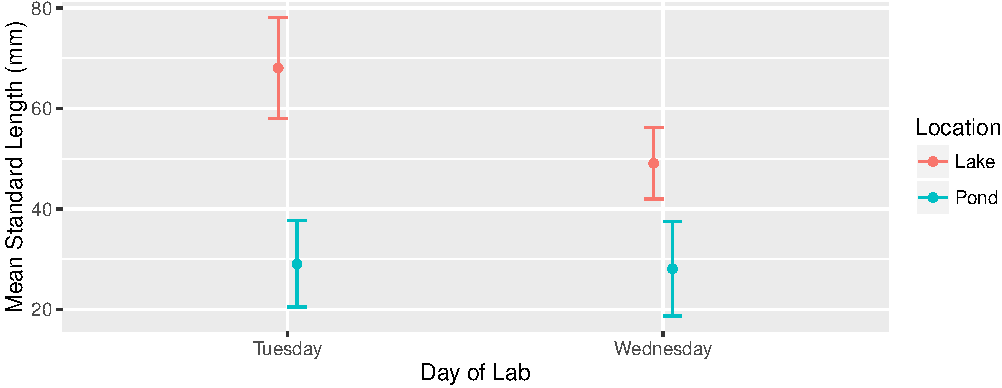
\includegraphics{skeleton_files/figure-latex/unnamed-chunk-45-1.pdf}

\begin{Shaded}
\begin{Highlighting}[]
\NormalTok{day_loc_summaries %>%}\StringTok{ }
\StringTok{  }\KeywordTok{ggplot}\NormalTok{(}\KeywordTok{aes}\NormalTok{(}\DataTypeTok{x =} \NormalTok{Location, }\DataTypeTok{y =} \NormalTok{mean, }\DataTypeTok{colour =} \NormalTok{Day_of_Lab)) +}
\StringTok{  }\KeywordTok{geom_errorbar}\NormalTok{(}\KeywordTok{aes}\NormalTok{(}\DataTypeTok{ymin =} \NormalTok{lower_CI_limit, }\DataTypeTok{ymax =} \NormalTok{upper_CI_limit), }
                \DataTypeTok{width =} \FloatTok{0.1}\NormalTok{, }\DataTypeTok{position =} \NormalTok{dodge) +}
\StringTok{  }\KeywordTok{geom_point}\NormalTok{(}\DataTypeTok{position =} \NormalTok{dodge) +}
\StringTok{  }\KeywordTok{xlab}\NormalTok{(}\StringTok{"Location"}\NormalTok{) +}\StringTok{ }\KeywordTok{ylab}\NormalTok{(}\StringTok{"Mean Standard Length (mm)"}\NormalTok{)}
\end{Highlighting}
\end{Shaded}

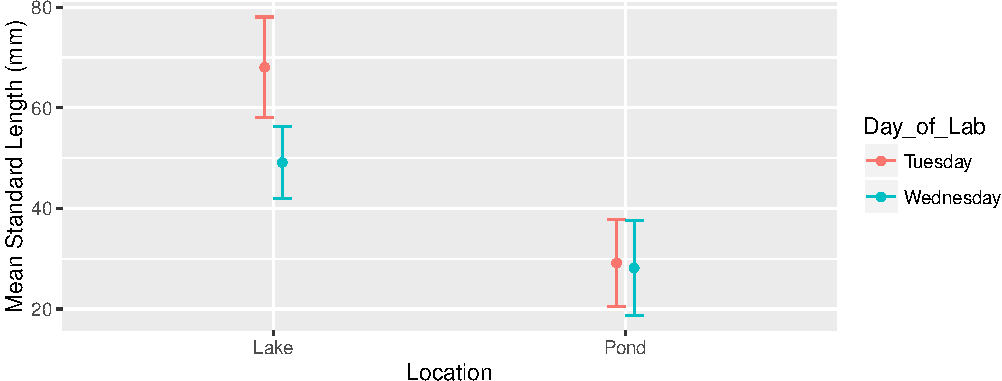
\includegraphics{skeleton_files/figure-latex/unnamed-chunk-46-1.pdf}

\section{How to Make an Overlay Plot}\label{how-to-make-an-overlay-plot}

This shows how to plot more than one line on a set of axes. An
appropriate data set for this type of analysis includes at least two
columns containing continuous \texttt{int} or \texttt{dbl} data that are
associated with each other row by row, and a column containing nominal
\texttt{chr} data that represent the different treatments.

First, the data is loaded in:

\begin{Shaded}
\begin{Highlighting}[]
\NormalTok{overlay <-}\StringTok{ }\KeywordTok{read_csv}\NormalTok{(}\StringTok{"data/overlay_data.csv"}\NormalTok{)}
\KeywordTok{str}\NormalTok{(overlay)}
\end{Highlighting}
\end{Shaded}

\begin{Verbatim}[frame=single]
Classes 'tbl_df', 'tbl' and 'data.frame':   14 obs. of  3 variables:
 $ Irradiance: int  1035 820 626 413 203 105 0 1038 821 617 ...
 $ PS_Rate   : num  4.56 4.25 3.78 2.78 1.31 ...
 $ species   : chr  "corn" "corn" "corn" "corn" ...
\end{Verbatim}

Then, a plot is made:

\begin{Shaded}
\begin{Highlighting}[]
\NormalTok{overlay %>%}\StringTok{ }
\StringTok{  }\KeywordTok{ggplot}\NormalTok{(}\KeywordTok{aes}\NormalTok{(}\DataTypeTok{x =} \NormalTok{Irradiance, }\DataTypeTok{y =} \NormalTok{PS_Rate, }\DataTypeTok{colour =} \NormalTok{species)) +}
\StringTok{  }\KeywordTok{geom_point}\NormalTok{(}\KeywordTok{aes}\NormalTok{(}\DataTypeTok{shape =} \NormalTok{species)) +}
\StringTok{  }\KeywordTok{geom_line}\NormalTok{()}
\end{Highlighting}
\end{Shaded}

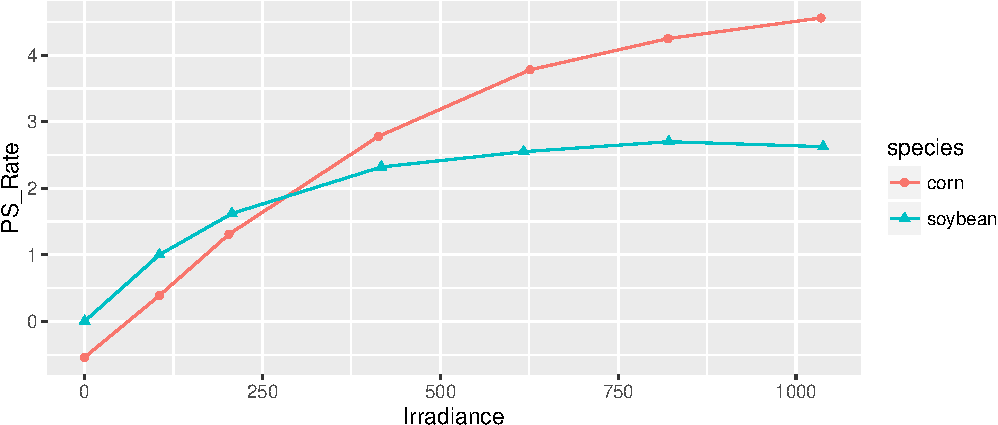
\includegraphics{skeleton_files/figure-latex/unnamed-chunk-48-1.pdf}

\section{How to Fit a Curve to a Y by X
Graph}\label{how-to-fit-a-curve-to-a-y-by-x-graph}

An appropriate data set for this type of analysis includes two columns
containing continuous \texttt{int} or \texttt{dbl} data that are
associated with each other row by row. For a relationship that is not
linear, it does not make sense to turn on the best-fit straight line or
the 95\% confidence intervals for the slope. Many types of curves can be
fit through bivariate data points. The \texttt{geom\_smooth} function
will be used here with \texttt{method\ =\ loess}, where ``loess'' is an
abbreviation for ``local polynomial regression fitting.''

\begin{Shaded}
\begin{Highlighting}[]
\NormalTok{X <-}\StringTok{ }\KeywordTok{c}\NormalTok{(}\FloatTok{1116.4}\NormalTok{, }\DecValTok{870}\NormalTok{, }\DecValTok{630}\NormalTok{, }\DecValTok{470}\NormalTok{, }\DecValTok{239}\NormalTok{, }\DecValTok{118}\NormalTok{, }\DecValTok{0}\NormalTok{)}
\NormalTok{Y <-}\StringTok{ }\KeywordTok{c}\NormalTok{(}\FloatTok{4.17}\NormalTok{, }\FloatTok{4.04}\NormalTok{, }\FloatTok{3.67}\NormalTok{, }\FloatTok{3.22}\NormalTok{, }\FloatTok{1.78}\NormalTok{, }\FloatTok{0.78}\NormalTok{, -}\FloatTok{0.49}\NormalTok{)}
\NormalTok{curve_data <-}\StringTok{ }\KeywordTok{data_frame}\NormalTok{(X, Y)}
\end{Highlighting}
\end{Shaded}

\begin{Shaded}
\begin{Highlighting}[]
\NormalTok{curve_data %>%}\StringTok{ }\KeywordTok{ggplot}\NormalTok{(}\KeywordTok{aes}\NormalTok{(}\DataTypeTok{x =} \NormalTok{X, }\DataTypeTok{y =} \NormalTok{Y)) +}
\StringTok{  }\KeywordTok{geom_point}\NormalTok{() +}
\StringTok{  }\KeywordTok{geom_smooth}\NormalTok{(}\DataTypeTok{method =} \StringTok{"loess"}\NormalTok{, }\DataTypeTok{se =} \OtherTok{FALSE}\NormalTok{)}
\end{Highlighting}
\end{Shaded}

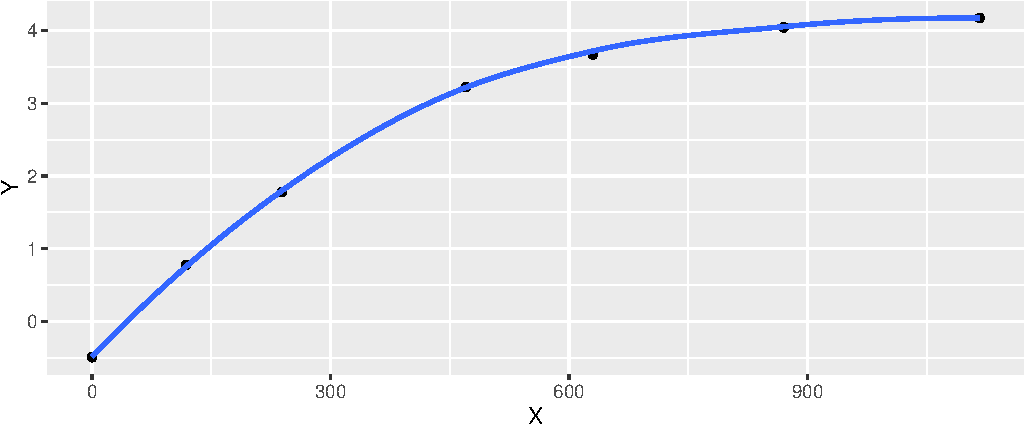
\includegraphics{skeleton_files/figure-latex/unnamed-chunk-50-1.pdf}

The \texttt{loess} method uses a default sensitivity \texttt{span} value
of 0.75. You can tweak this value as you see fit to control the degree
of smoothing. A few examples are below.

\begin{Shaded}
\begin{Highlighting}[]
\NormalTok{curve_data %>%}\StringTok{ }\KeywordTok{ggplot}\NormalTok{(}\KeywordTok{aes}\NormalTok{(}\DataTypeTok{x =} \NormalTok{X, }\DataTypeTok{y =} \NormalTok{Y)) +}
\StringTok{  }\KeywordTok{geom_point}\NormalTok{() +}
\StringTok{  }\KeywordTok{geom_smooth}\NormalTok{(}\DataTypeTok{method =} \StringTok{"loess"}\NormalTok{, }\DataTypeTok{se =} \OtherTok{FALSE}\NormalTok{, }\DataTypeTok{span =} \DecValTok{1000}\NormalTok{)}
\end{Highlighting}
\end{Shaded}

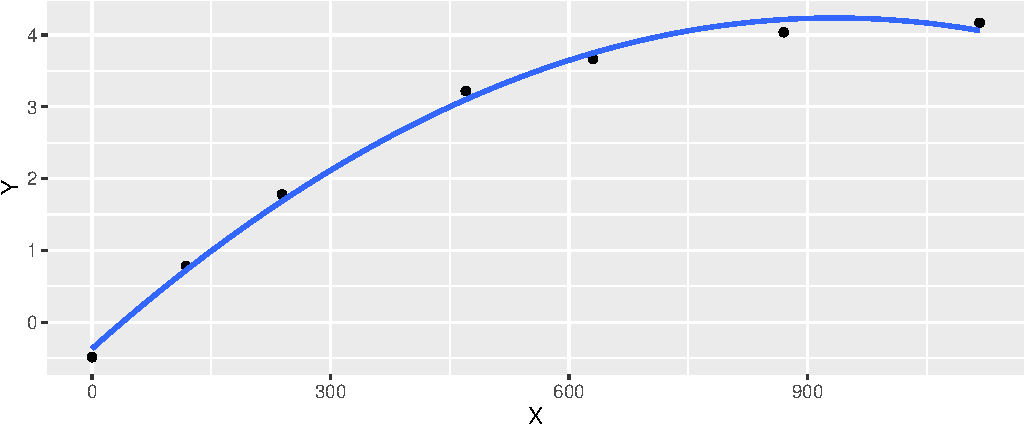
\includegraphics{skeleton_files/figure-latex/unnamed-chunk-51-1.pdf}

\begin{Shaded}
\begin{Highlighting}[]
\NormalTok{curve_data %>%}\StringTok{ }\KeywordTok{ggplot}\NormalTok{(}\KeywordTok{aes}\NormalTok{(}\DataTypeTok{x =} \NormalTok{X, }\DataTypeTok{y =} \NormalTok{Y)) +}
\StringTok{  }\KeywordTok{geom_point}\NormalTok{() +}
\StringTok{  }\KeywordTok{geom_smooth}\NormalTok{(}\DataTypeTok{method =} \StringTok{"loess"}\NormalTok{, }\DataTypeTok{se =} \OtherTok{FALSE}\NormalTok{, }\DataTypeTok{span =} \FloatTok{0.6}\NormalTok{)}
\end{Highlighting}
\end{Shaded}

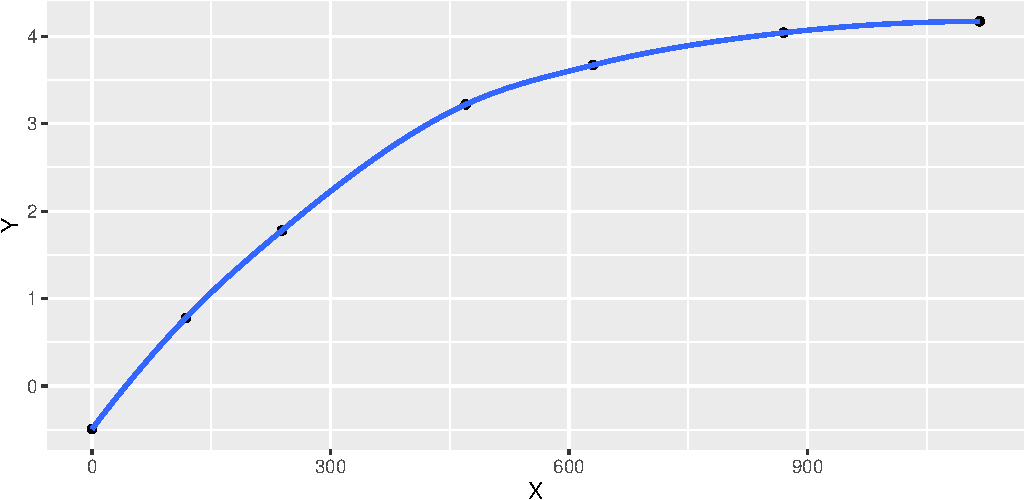
\includegraphics{skeleton_files/figure-latex/unnamed-chunk-52-1.pdf}

You can also add reference lines to plots by using the
\texttt{geom\_hline} and \texttt{geom\_vline} functions. These vertical
lines may be useful to find the X value where the fit curve crosses the
X-axis or to find the X value where the fit curve levels off.

\begin{Shaded}
\begin{Highlighting}[]
\NormalTok{curve_data %>%}\StringTok{ }\KeywordTok{ggplot}\NormalTok{(}\KeywordTok{aes}\NormalTok{(}\DataTypeTok{x =} \NormalTok{X, }\DataTypeTok{y =} \NormalTok{Y)) +}
\StringTok{  }\KeywordTok{geom_point}\NormalTok{() +}
\StringTok{  }\KeywordTok{geom_smooth}\NormalTok{(}\DataTypeTok{method =} \StringTok{"loess"}\NormalTok{, }\DataTypeTok{se =} \OtherTok{FALSE}\NormalTok{, }\DataTypeTok{colour =} \StringTok{"red"}\NormalTok{) +}
\StringTok{  }\KeywordTok{geom_hline}\NormalTok{(}\DataTypeTok{yintercept =} \DecValTok{0}\NormalTok{) +}
\StringTok{  }\KeywordTok{geom_vline}\NormalTok{(}\DataTypeTok{xintercept =} \DecValTok{900}\NormalTok{, }\DataTypeTok{colour =} \StringTok{"blue"}\NormalTok{) +}
\StringTok{  }\KeywordTok{geom_vline}\NormalTok{(}\DataTypeTok{xintercept =} \DecValTok{50}\NormalTok{, }\DataTypeTok{colour =} \StringTok{"blue"}\NormalTok{)}
\end{Highlighting}
\end{Shaded}

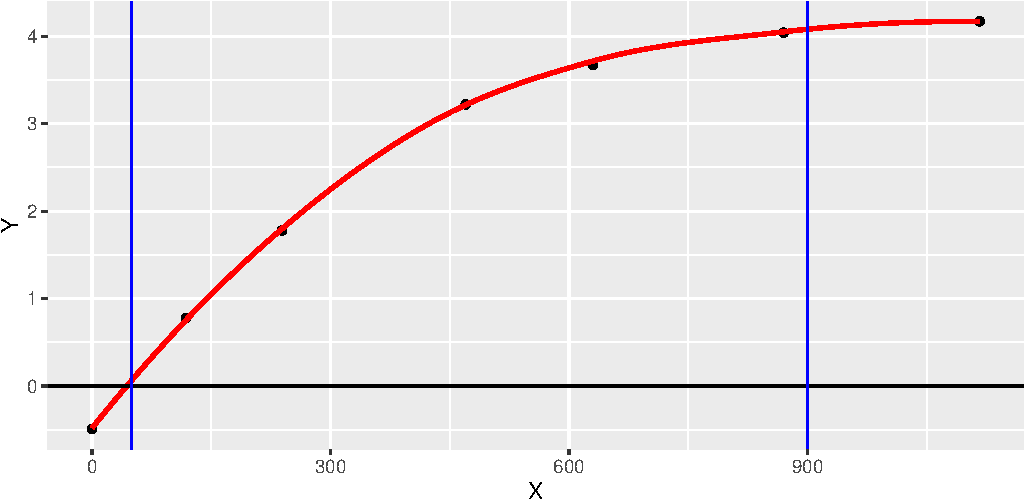
\includegraphics{skeleton_files/figure-latex/unnamed-chunk-53-1.pdf}

\section{\texorpdfstring{Testing the Difference Between \textbf{Two}
Means (unpaired
data)}{Testing the Difference Between Two Means (unpaired data)}}\label{testing-the-difference-between-two-means-unpaired-data}

An appropriate data set for this type of analysis contains at least one
column that designates the experimental condition as a nominal
\texttt{chr} variable X and one column that contains the Y response
variable as continuous \texttt{int} or \texttt{dbl} data.

First, the data is loaded:

\begin{Shaded}
\begin{Highlighting}[]
\NormalTok{unpaired_data <-}\StringTok{ }\KeywordTok{read_csv}\NormalTok{(}\StringTok{"data/unpaired.csv"}\NormalTok{)}
\end{Highlighting}
\end{Shaded}

Next a \texttt{t.test} is performed. Note that the \textbf{t test} only
works when comparing the mean measurements of exactly two groups and
assuming the variances of the two population groups are equal. (There is
a separate \textbf{t test} option that assumes unequal variances.)

\begin{Shaded}
\begin{Highlighting}[]
\KeywordTok{t.test}\NormalTok{(bp ~}\StringTok{ }\NormalTok{drug, }\DataTypeTok{data =} \NormalTok{unpaired_data, }\DataTypeTok{var.equal =} \OtherTok{TRUE}\NormalTok{)}
\end{Highlighting}
\end{Shaded}

\begin{Verbatim}[frame=single]

    Two Sample t-test

data:  bp by drug
t = 0.57438, df = 8, p-value = 0.5815
alternative hypothesis: true difference in means is not equal to 0
95 percent confidence interval:
 -9.044319 15.044319
sample estimates:
mean in group A mean in group B 
          130.2           127.2 
\end{Verbatim}

\begin{itemize}
\tightlist
\item
  Here, the \texttt{p-value} is the same as the ANOVA
  \texttt{Pr(\textgreater{}F)} p-value given below. The \textbf{ANOVA}
  model is the extension of the equal variance \textbf{t test}.
\end{itemize}

\begin{Shaded}
\begin{Highlighting}[]
\KeywordTok{anova}\NormalTok{(}\KeywordTok{aov}\NormalTok{(bp ~}\StringTok{ }\NormalTok{drug, }\DataTypeTok{data =} \NormalTok{unpaired_data))}
\end{Highlighting}
\end{Shaded}

\begin{Verbatim}[frame=single]
Analysis of Variance Table

Response: bp
          Df Sum Sq Mean Sq F value Pr(>F)
drug       1   22.5    22.5  0.3299 0.5815
Residuals  8  545.6    68.2               
\end{Verbatim}

It's often appropriate to compare the distributions of response values
for the two groups. This is most frequently done by comparing boxplots
as below:

\begin{Shaded}
\begin{Highlighting}[]
\NormalTok{unpaired_data %>%}\StringTok{ }\KeywordTok{ggplot}\NormalTok{(}\KeywordTok{aes}\NormalTok{(}\DataTypeTok{x =} \NormalTok{drug, }\DataTypeTok{y =} \NormalTok{bp)) +}
\StringTok{  }\KeywordTok{geom_boxplot}\NormalTok{()}
\end{Highlighting}
\end{Shaded}

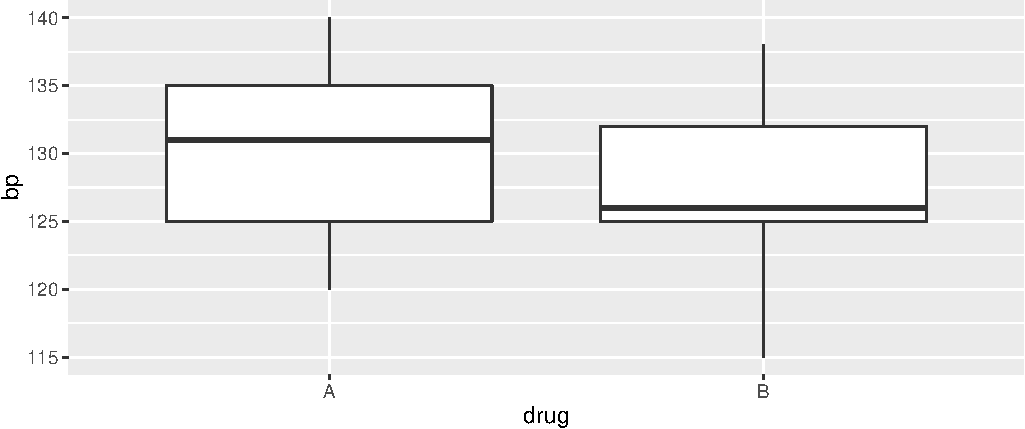
\includegraphics{skeleton_files/figure-latex/unnamed-chunk-57-1.pdf}

See page I-11 for more explanation.

\section{\texorpdfstring{Testing the Difference Between \textbf{Two}
Means (paired
data)}{Testing the Difference Between Two Means (paired data)}}\label{testing-the-difference-between-two-means-paired-data}

\begin{itemize}
\item
  Data are considered paired if they are dependent in some way. This
  could be a male and female in a pair, or the same individual tested
  over time or under different conditions as in before and after taking
  a drug.
\item
  There are two formats with which paired data often is stored. You can
  convert the second format into the first as you will see later.
\end{itemize}

\subsubsection*{FORMAT 1}\label{format-1}
\addcontentsline{toc}{subsubsection}{FORMAT 1}

\begin{figure}[htbp]
\centering
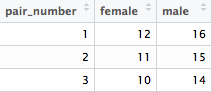
\includegraphics{figure/format1.png}
\caption{Format 1}
\end{figure}

\begin{itemize}
\tightlist
\item
  Here the data includes \textbf{two} columns containing the two
  measures of the continuous variable such that paired data for each are
  on a single row. Again, the \texttt{t.test} function is used but this
  time we specify \texttt{paired\ =\ TRUE}. (It is set to \texttt{FALSE}
  by default.)
\end{itemize}

\begin{Shaded}
\begin{Highlighting}[]
\NormalTok{pair_number <-}\StringTok{ }\KeywordTok{c}\NormalTok{(}\DecValTok{1}\NormalTok{:}\DecValTok{10}\NormalTok{)}
\NormalTok{female <-}\StringTok{ }\KeywordTok{c}\NormalTok{(}\DecValTok{12}\NormalTok{, }\DecValTok{11}\NormalTok{, }\DecValTok{10}\NormalTok{, }\DecValTok{9}\NormalTok{, }\DecValTok{8}\NormalTok{, }\DecValTok{7}\NormalTok{, }\DecValTok{6}\NormalTok{, }\DecValTok{5}\NormalTok{, }\DecValTok{4}\NormalTok{, }\DecValTok{3}\NormalTok{)}
\NormalTok{male <-}\StringTok{ }\KeywordTok{c}\NormalTok{(}\DecValTok{16}\NormalTok{, }\DecValTok{15}\NormalTok{, }\DecValTok{14}\NormalTok{, }\DecValTok{13}\NormalTok{, }\DecValTok{10}\NormalTok{, }\DecValTok{9}\NormalTok{, }\DecValTok{8}\NormalTok{, }\DecValTok{6}\NormalTok{, }\DecValTok{5}\NormalTok{, }\DecValTok{3}\NormalTok{)}
\NormalTok{matched_df <-}\StringTok{ }\KeywordTok{data_frame}\NormalTok{(pair_number, female, male)}
\KeywordTok{t.test}\NormalTok{(matched_df$female, matched_df$male, }\DataTypeTok{paired =} \OtherTok{TRUE}\NormalTok{)}
\end{Highlighting}
\end{Shaded}

\begin{Verbatim}[frame=single]

    Paired t-test

data:  matched_df$female and matched_df$male
t = -5.041, df = 9, p-value = 0.0006988
alternative hypothesis: true difference in means is not equal to 0
95 percent confidence interval:
 -3.477002 -1.322998
sample estimates:
mean of the differences 
                   -2.4 
\end{Verbatim}

\begin{itemize}
\item
  The \texttt{p-value} here is for the paired t-test with the null
  hypothesis that there is no significant difference between the means
  of the two populations.
\item
  If you use the \texttt{paired\ =\ TRUE} option, \texttt{t.test}
  expects the data to be stored as vectors and that's why the
  \texttt{\$} syntax is used as opposed to the usual \texttt{formula}
  syntax.
\item
  Next a plot of the difference of the two responses is on the y-axis,
  and the mean of the two responses on the x-axis. Additionally, lines
  have been added for the lower and upper bounds of a 95\% confidence
  interval for the population mean difference as well as the sample mean
  difference, which are calculated in the \texttt{summary\_matched}
  variable.
\end{itemize}

\begin{Shaded}
\begin{Highlighting}[]
\NormalTok{matched_1 <-}\StringTok{ }\NormalTok{matched_df %>%}
\StringTok{  }\KeywordTok{mutate}\NormalTok{(}\DataTypeTok{difference =} \NormalTok{male -}\StringTok{ }\NormalTok{female,}
         \DataTypeTok{avg =} \NormalTok{(male +}\StringTok{ }\NormalTok{female) /}\StringTok{ }\DecValTok{2}\NormalTok{)}
\KeywordTok{str}\NormalTok{(matched_1)}
\end{Highlighting}
\end{Shaded}

\begin{Verbatim}[frame=single]
Classes 'tbl_df', 'tbl' and 'data.frame':   10 obs. of  5 variables:
 $ pair_number: int  1 2 3 4 5 6 7 8 9 10
 $ female     : num  12 11 10 9 8 7 6 5 4 3
 $ male       : num  16 15 14 13 10 9 8 6 5 3
 $ difference : num  4 4 4 4 2 2 2 1 1 0
 $ avg        : num  14 13 12 11 9 8 7 5.5 4.5 3
\end{Verbatim}

\begin{Shaded}
\begin{Highlighting}[]
\NormalTok{summary_matched <-}\StringTok{ }\NormalTok{matched_1 %>%}
\StringTok{  }\KeywordTok{summarize}\NormalTok{(}\DataTypeTok{mean =} \KeywordTok{mean}\NormalTok{(difference),}
            \DataTypeTok{std_dev =} \KeywordTok{sd}\NormalTok{(difference),}
            \DataTypeTok{N =} \KeywordTok{n}\NormalTok{(),}
            \DataTypeTok{std_err =} \NormalTok{std_dev /}\StringTok{ }\KeywordTok{sqrt}\NormalTok{(N),}
            \DataTypeTok{lower_CI_limit =} \NormalTok{mean +}\StringTok{ }\KeywordTok{qt}\NormalTok{(}\FloatTok{0.025}\NormalTok{, }\DataTypeTok{df =} \NormalTok{N}\DecValTok{-1}\NormalTok{) *}\StringTok{ }\NormalTok{std_err,}
            \DataTypeTok{upper_CI_limit =} \NormalTok{mean +}\StringTok{ }\KeywordTok{qt}\NormalTok{(}\FloatTok{0.975}\NormalTok{, }\DataTypeTok{df =} \NormalTok{N}\DecValTok{-1}\NormalTok{) *}\StringTok{ }\NormalTok{std_err) }
\end{Highlighting}
\end{Shaded}

\begin{Shaded}
\begin{Highlighting}[]
\NormalTok{matched_1 %>%}\StringTok{ }\KeywordTok{ggplot}\NormalTok{(}\KeywordTok{aes}\NormalTok{(}\DataTypeTok{x =} \NormalTok{avg, }\DataTypeTok{y =} \NormalTok{difference)) +}
\StringTok{  }\KeywordTok{geom_point}\NormalTok{() +}
\StringTok{  }\KeywordTok{geom_hline}\NormalTok{(}\DataTypeTok{yintercept =} \NormalTok{summary_matched$lower_CI_limit, }
             \DataTypeTok{linetype =} \StringTok{"dashed"}\NormalTok{, }\DataTypeTok{colour =} \StringTok{"red"}\NormalTok{) +}
\StringTok{  }\KeywordTok{geom_hline}\NormalTok{(}\DataTypeTok{yintercept =} \NormalTok{summary_matched$upper_CI_limit, }
             \DataTypeTok{linetype =} \StringTok{"dashed"}\NormalTok{, }\DataTypeTok{colour =} \StringTok{"red"}\NormalTok{) +}\StringTok{ }
\StringTok{  }\KeywordTok{geom_hline}\NormalTok{(}\DataTypeTok{yintercept =} \NormalTok{summary_matched$mean, }
             \DataTypeTok{colour =} \StringTok{"red"}\NormalTok{)}
\end{Highlighting}
\end{Shaded}

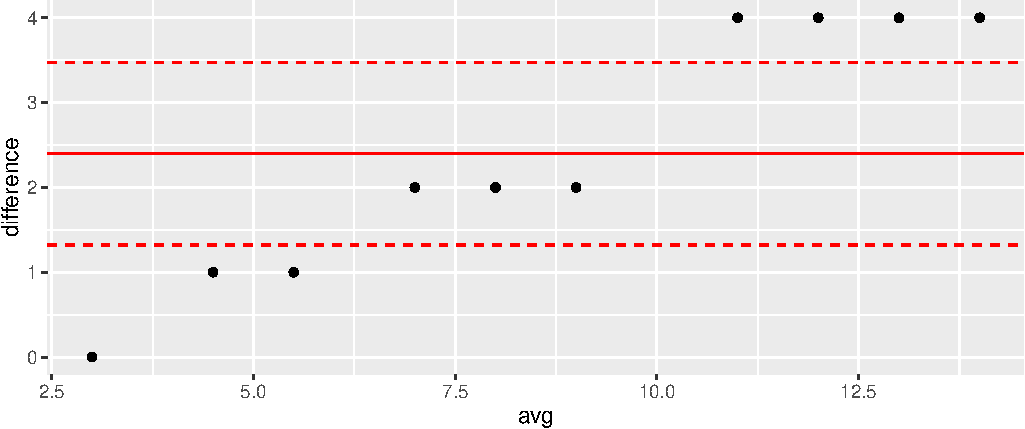
\includegraphics{skeleton_files/figure-latex/unnamed-chunk-61-1.pdf}

\subsubsection*{FORMAT 2}\label{format-2}
\addcontentsline{toc}{subsubsection}{FORMAT 2}

\begin{figure}[htbp]
\centering
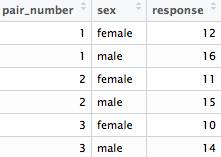
\includegraphics{figure/format2.png}
\caption{Format 2}
\end{figure}

\begin{itemize}
\tightlist
\item
  Here the data includes \textbf{one} column containing the continuous
  variable that you have measured as the response variable
  (\texttt{response} above), a second column that designates the
  experimental condition as a nominal column (\texttt{sex} above), and a
  third column that designates how the data are paired
  (\texttt{pair\ number} above).
\end{itemize}

You can use the \texttt{spread} function in the \texttt{tidyr} package
to transform data of this form into the format seen in \textbf{FORMAT
1}:

\begin{Shaded}
\begin{Highlighting}[]
\NormalTok{matched_2 <-}\StringTok{ }\KeywordTok{read_csv}\NormalTok{(}\StringTok{"data/matched2.csv"}\NormalTok{)}
\NormalTok{matched_spread <-}\StringTok{ }\NormalTok{matched_2 %>%}\StringTok{ }\KeywordTok{spread}\NormalTok{(}\DataTypeTok{key =} \NormalTok{sex, }\DataTypeTok{value =} \NormalTok{response)}
\KeywordTok{str}\NormalTok{(matched_spread)}
\end{Highlighting}
\end{Shaded}

\begin{Verbatim}[frame=single]
Classes 'tbl_df', 'tbl' and 'data.frame':   10 obs. of  3 variables:
 $ pair_number: int  1 2 3 4 5 6 7 8 9 10
 $ female     : int  12 11 10 9 8 7 6 5 4 3
 $ male       : int  16 15 14 13 10 9 8 6 5 3
\end{Verbatim}

The same results as before are given since the data sets
(\texttt{matched\_spread} and \texttt{matched\_df}) now match:

\begin{Shaded}
\begin{Highlighting}[]
\KeywordTok{t.test}\NormalTok{(matched_spread$female, matched_spread$male, }\DataTypeTok{paired =} \OtherTok{TRUE}\NormalTok{)}
\end{Highlighting}
\end{Shaded}

\begin{Verbatim}[frame=single]

    Paired t-test

data:  matched_spread$female and matched_spread$male
t = -5.041, df = 9, p-value = 0.0006988
alternative hypothesis: true difference in means is not equal to 0
95 percent confidence interval:
 -3.477002 -1.322998
sample estimates:
mean of the differences 
                   -2.4 
\end{Verbatim}

A useful plot can be created that connects members of pairs by their
response values if data is of the \textbf{FORMAT 2} variety. If you'd
like to transfer data in \textbf{FORMAT 1} into \textbf{FORMAT 2}, you
can use the \texttt{gather} function which is essentially the opposite
of the \texttt{spread} function.

\begin{Shaded}
\begin{Highlighting}[]
\NormalTok{matched_gather <-}\StringTok{ }\NormalTok{matched_spread %>%}
\StringTok{  }\KeywordTok{gather}\NormalTok{(}\DataTypeTok{key =} \NormalTok{sex, }\DataTypeTok{value =} \NormalTok{response, -pair_number)}
\NormalTok{matched_gather}
\end{Highlighting}
\end{Shaded}

\begin{Verbatim}[frame=single]
Source: local data frame [20 x 3]

   pair_number    sex response
         <int>  <chr>    <int>
1            1 female       12
2            2 female       11
3            3 female       10
4            4 female        9
5            5 female        8
6            6 female        7
7            7 female        6
8            8 female        5
9            9 female        4
10          10 female        3
11           1   male       16
12           2   male       15
13           3   male       14
14           4   male       13
15           5   male       10
16           6   male        9
17           7   male        8
18           8   male        6
19           9   male        5
20          10   male        3
\end{Verbatim}

\begin{Shaded}
\begin{Highlighting}[]
\NormalTok{matched_gather %>%}\StringTok{ }\KeywordTok{ggplot}\NormalTok{(}\KeywordTok{aes}\NormalTok{(}\DataTypeTok{x =} \NormalTok{sex, }\DataTypeTok{y =} \NormalTok{response, }
                              \DataTypeTok{colour =} \KeywordTok{factor}\NormalTok{(pair_number))) +}
\StringTok{  }\KeywordTok{geom_point}\NormalTok{() +}
\StringTok{  }\KeywordTok{geom_line}\NormalTok{(}\KeywordTok{aes}\NormalTok{(}\DataTypeTok{group =} \NormalTok{pair_number))}
\end{Highlighting}
\end{Shaded}

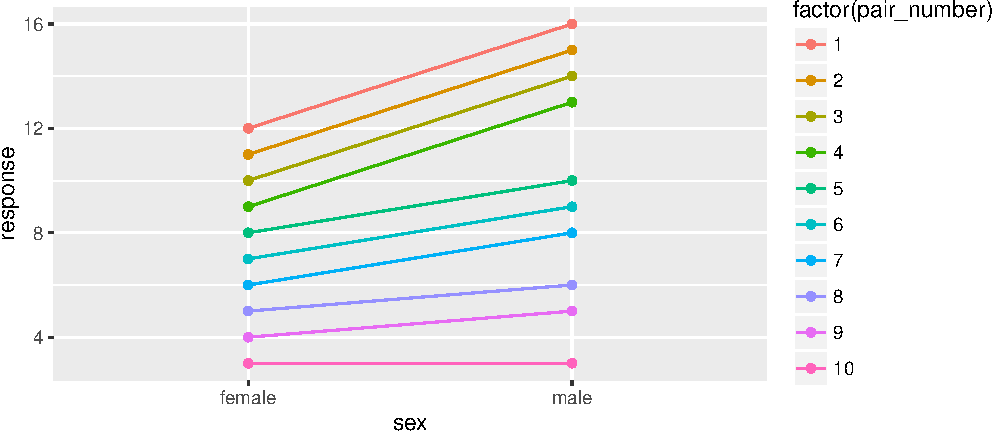
\includegraphics{skeleton_files/figure-latex/unnamed-chunk-64-1.pdf}

The addition of \texttt{factor()} here is done so that the pair numbers
are treated as categories and not as a continuous variable to better
differentiate the colors. Without the \texttt{factor} addition, the
colors will correspond to different shadings of the default color blue
with 10 corresponding to darkest and 1 corresponding to lightest.

Summary information can also be provided via the following:

\begin{Shaded}
\begin{Highlighting}[]
\NormalTok{matched_gather %>%}\StringTok{ }
\StringTok{  }\KeywordTok{group_by}\NormalTok{(sex) %>%}
\StringTok{  }\KeywordTok{summarize}\NormalTok{(}\DataTypeTok{mean =} \KeywordTok{mean}\NormalTok{(response),}
            \DataTypeTok{std_dev =} \KeywordTok{sd}\NormalTok{(response),}
            \DataTypeTok{N =} \KeywordTok{n}\NormalTok{(),}
            \DataTypeTok{std_err =} \NormalTok{std_dev /}\StringTok{ }\KeywordTok{sqrt}\NormalTok{(N),}
            \DataTypeTok{lower_CI_limit =} \NormalTok{mean +}\StringTok{ }\KeywordTok{qt}\NormalTok{(}\FloatTok{0.025}\NormalTok{, }\DataTypeTok{df =} \NormalTok{N}\DecValTok{-1}\NormalTok{) *}\StringTok{ }\NormalTok{std_err,}
            \DataTypeTok{upper_CI_limit =} \NormalTok{mean +}\StringTok{ }\KeywordTok{qt}\NormalTok{(}\FloatTok{0.975}\NormalTok{, }\DataTypeTok{df =} \NormalTok{N}\DecValTok{-1}\NormalTok{) *}\StringTok{ }\NormalTok{std_err) }
\end{Highlighting}
\end{Shaded}

\begin{Verbatim}[frame=single]
Source: local data frame [2 x 7]

     sex  mean  std_dev     N   std_err lower_CI_limit upper_CI_limit
   <chr> <dbl>    <dbl> <int>     <dbl>          <dbl>          <dbl>
1 female   7.5 3.027650    10 0.9574271       5.334149       9.665851
2   male   9.9 4.483302    10 1.4177447       6.692839      13.107161
\end{Verbatim}

\begin{itemize}
\tightlist
\item
  This format and test can be expanded to more than two groups (ex:
  response of each individual to 3 different drugs) for a
  \textbf{repeated measures ANOVA}.
\end{itemize}

\section{Equivalence Test}\label{equivalence-test}

An appropriate data set for this type of analysis contains at least one
column that designates the experimental condition as a nominal
\texttt{chr} variable X and one column that contains the Y response
variable as continuous \texttt{int} or \texttt{dbl} data.

\begin{itemize}
\item
  You want to confirm that there is no significant difference in mean Y
  response variable for the different X experimental conditions, but it
  is impossible to prove this.
\item
  Instead, you need to pick a threshold of difference for which any
  smaller differences are considered to be irrelevant. This threshold
  can be set based on the limits of technical resolution or practical
  importance.
\item
  The \textbf{Equivalence Test} in R uses two \textbf{\emph{t}-tests} to
  determine if the difference between the two means of interest is
  significantly different from the allowed threshold of difference,
  denoted by \texttt{epsilon} (\(\varepsilon\)).
\end{itemize}

\begin{Shaded}
\begin{Highlighting}[]
\NormalTok{equivalence::}\KeywordTok{tost}\NormalTok{(matched_spread$male, matched_spread$female, }
                  \DataTypeTok{epsilon =} \DecValTok{6}\NormalTok{)}
\end{Highlighting}
\end{Shaded}

\begin{Verbatim}[frame=single]

    Welch Two Sample TOST

data:  matched_spread$male and matched_spread$female
df = 15.796
sample estimates:
mean of x mean of y 
      9.9       7.5 
\end{Verbatim}

See page I-12 for more explanation.

\section{Chi-Square Contingency Table
Analysis}\label{chi-square-contingency-table-analysis}

\subsection*{For raw data that need to be
tallied}\label{for-raw-data-that-need-to-be-tallied}
\addcontentsline{toc}{subsection}{For raw data that need to be tallied}

An appropriate data set for this type of analysis contains at least two
columns containing nominal \texttt{chr} variables.

\begin{Shaded}
\begin{Highlighting}[]
\NormalTok{nom_data <-}\StringTok{ }\KeywordTok{read_csv}\NormalTok{(}\StringTok{"data/contingency.csv"}\NormalTok{)}
\KeywordTok{str}\NormalTok{(nom_data)}
\end{Highlighting}
\end{Shaded}

\begin{Verbatim}[frame=single]
Classes 'tbl_df', 'tbl' and 'data.frame':   32 obs. of  2 variables:
 $ sex  : chr  "F" "M" "M" "F" ...
 $ color: chr  "blue" "red" "green" "green" ...
\end{Verbatim}

To visualize this data we can do the following:

\begin{Shaded}
\begin{Highlighting}[]
\NormalTok{colors =}\StringTok{ }\KeywordTok{c}\NormalTok{(}\DataTypeTok{blue =} \StringTok{"blue"}\NormalTok{, }\DataTypeTok{red =} \StringTok{"red"}\NormalTok{, }\DataTypeTok{green =} \StringTok{"forestgreen"}\NormalTok{)}
\NormalTok{nom_data %>%}\StringTok{ }\KeywordTok{ggplot}\NormalTok{(}\KeywordTok{aes}\NormalTok{(}\DataTypeTok{x =} \NormalTok{sex, }\DataTypeTok{fill =} \NormalTok{color)) +}\StringTok{ }
\StringTok{  }\KeywordTok{geom_bar}\NormalTok{(}\DataTypeTok{position =} \StringTok{"fill"}\NormalTok{) +}
\StringTok{  }\KeywordTok{scale_fill_manual}\NormalTok{(}\DataTypeTok{values =} \NormalTok{colors) +}\StringTok{ }
\StringTok{  }\KeywordTok{ylab}\NormalTok{(}\StringTok{"portion"}\NormalTok{)}
\end{Highlighting}
\end{Shaded}

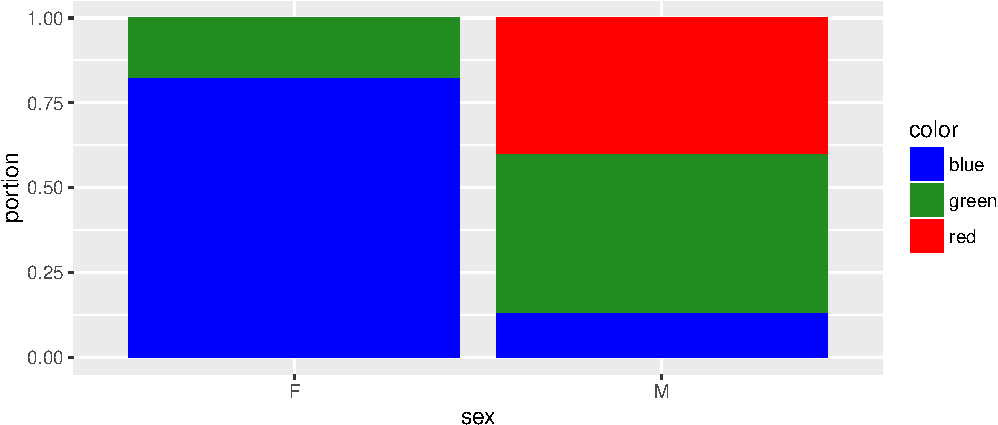
\includegraphics{skeleton_files/figure-latex/unnamed-chunk-68-1.pdf}

You want to examine the distribution of a nominal response variable
(\texttt{color} above) that you measured as predicted by the values of a
nominal (\texttt{sex} above) that you have imposed or occurred
naturally. Note that both Y and X may contain \textgreater{}2
categories.

First, you'll need to tally the data and you can use the
\texttt{table()} function to do so:

\begin{Shaded}
\begin{Highlighting}[]
\NormalTok{contin_table <-}\StringTok{ }\KeywordTok{table}\NormalTok{(nom_data)}
\NormalTok{contin_table}
\end{Highlighting}
\end{Shaded}

\begin{Verbatim}[frame=single]
   color
sex blue green red
  F   14     3   0
  M    2     7   6
\end{Verbatim}

The observed total for each cell is tallied from the data table and
appears in the upper right hand corner of each cell on the contingency
table (always integers). You then pass this \texttt{table} object, which
is essentially just a 2 x 3 matrix containing the count values, into the
\texttt{chisq.test} function:

\begin{Shaded}
\begin{Highlighting}[]
\NormalTok{chi_square_test <-}\StringTok{ }\KeywordTok{chisq.test}\NormalTok{(contin_table)}
\end{Highlighting}
\end{Shaded}

\begin{Verbatim}[frame=single, formatcom=\color{red}]
Warning in chisq.test(contin_table): Chi-squared approximation may be
incorrect
\end{Verbatim}

\begin{Shaded}
\begin{Highlighting}[]
\NormalTok{chi_square_test}
\end{Highlighting}
\end{Shaded}

\begin{Verbatim}[frame=single]

    Pearson's Chi-squared test

data:  contin_table
X-squared = 16.54, df = 2, p-value = 0.0002561
\end{Verbatim}

The \texttt{p-value} here is used to decide if the null hypothesis can
be rejected.

The \(\chi^2\) test here produces a warning highlighted in red. To
better understand this warning, it's useful to look at the expected cell
counts. There are BIAS RULES which are assumptions that need to be
checked in order for the chi-square test to be unbiased:

\begin{enumerate}
\def\labelenumi{\arabic{enumi}.}
\item
  No expected frequency should be less than 1.0.
\item
  No more than 20\% of the expected frequencies should be less than 5.0.
\end{enumerate}

If your data violate the above bias rules, then the Chi-Square that you
calculate will be biased and may increase the probability of rejecting
\(H_0\) when it is actually true.

\begin{Shaded}
\begin{Highlighting}[]
\NormalTok{chi_square_test$expected}
\end{Highlighting}
\end{Shaded}

\begin{Verbatim}[frame=single]
   color
sex blue  green    red
  F  8.5 5.3125 3.1875
  M  7.5 4.6875 2.8125
\end{Verbatim}

You may also be interested in the column and row margin totals for your
contingency table. These can be added by wrapping the table in the
\texttt{addmargins} function. The row totals (far right) and column
totals (bottom row), as well as the grand total (lower right cell) are
given. These totals are used to calculate, for each cell, the value
expected if the null hypothesis is true. The expected values are
displayed above.

\begin{Shaded}
\begin{Highlighting}[]
\KeywordTok{addmargins}\NormalTok{(contin_table)}
\end{Highlighting}
\end{Shaded}

\begin{Verbatim}[frame=single]
     color
sex   blue green red Sum
  F     14     3   0  17
  M      2     7   6  15
  Sum   16    10   6  32
\end{Verbatim}

\emph{Important note}: Make sure not to run the \texttt{chisq.test}
procedure on a table that include margin totals since it will add those
into the analysis.

Another way to view the contingency table instead of by counts as
\texttt{table} provides is by using \texttt{prop.table()} function which
expects a \texttt{table} as input:

\begin{Shaded}
\begin{Highlighting}[]
\KeywordTok{prop.table}\NormalTok{(contin_table)}
\end{Highlighting}
\end{Shaded}

\begin{Verbatim}[frame=single]
   color
sex    blue   green     red
  F 0.43750 0.09375 0.00000
  M 0.06250 0.21875 0.18750
\end{Verbatim}

See page I-13 for more explanation.

\subsection*{For Tallied Results}\label{for-tallied-results}
\addcontentsline{toc}{subsection}{For Tallied Results}

An appropriate data set includes two nominal (\texttt{chr}) columns for
the two types of categories and a third with continuous (\texttt{int})
data showing the total number of times each combination occurred.

\begin{itemize}
\item
  For the counts, never use percentages as sample size is then lost.
\item
  Always use frequencies (the number of times something happened).
\end{itemize}

\begin{figure}[htbp]
\centering
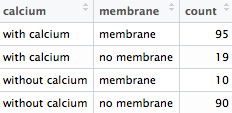
\includegraphics{figure/tallied.png}
\caption{Tallied}
\end{figure}

\begin{Shaded}
\begin{Highlighting}[]
\NormalTok{tallied <-}\StringTok{ }\KeywordTok{read_csv}\NormalTok{(}\StringTok{"data/tallied.csv"}\NormalTok{)}
\NormalTok{tallied}
\end{Highlighting}
\end{Shaded}

\begin{Verbatim}[frame=single]
Source: local data frame [4 x 3]

          calcium    membrane count
            <chr>       <chr> <int>
1    with calcium    membrane    95
2    with calcium no membrane    19
3 without calcium    membrane    10
4 without calcium no membrane    90
\end{Verbatim}

The \texttt{xtabs} functions turns this data frame into a contingency
table. The frequency goes to the left of the \texttt{\textasciitilde{}}
and the two nominal variables go to the right of the
\texttt{\textasciitilde{}} and are separated by a \texttt{+}. Lastly, we
include the \texttt{data} argument.

\begin{Shaded}
\begin{Highlighting}[]
\NormalTok{contin_table2 <-}\StringTok{ }\KeywordTok{xtabs}\NormalTok{(count ~}\StringTok{ }\NormalTok{calcium +}\StringTok{ }\NormalTok{membrane, }\DataTypeTok{data =} \NormalTok{tallied)}
\KeywordTok{chisq.test}\NormalTok{(contin_table2)}
\end{Highlighting}
\end{Shaded}

\begin{Verbatim}[frame=single]

    Pearson's Chi-squared test with Yates' continuity correction

data:  contin_table2
X-squared = 111.72, df = 1, p-value < 2.2e-16
\end{Verbatim}

See page I-13 for more explanation.

\section{Chi-Square Goodness of Fit
Analysis}\label{chi-square-goodness-of-fit-analysis}

An appropriately formatted data set includes one nominal column
containing categorical data such as male or female, heads or tails for a
coin toss, or A or a phenotype. You want to examine the distribution of
a nominal response variable Y that you measured as predicted by the
values of a theoretical model.

\begin{Shaded}
\begin{Highlighting}[]
\NormalTok{Phenotype <-}\StringTok{ }\KeywordTok{c}\NormalTok{(}\StringTok{"A"}\NormalTok{, }\StringTok{"A"}\NormalTok{, }\StringTok{"a"}\NormalTok{, }\StringTok{"A"}\NormalTok{, }\StringTok{"A"}\NormalTok{, }\StringTok{"A"}\NormalTok{, }\StringTok{"A"}\NormalTok{,}
               \StringTok{"a"}\NormalTok{, }\StringTok{"A"}\NormalTok{, }\StringTok{"a"}\NormalTok{, }\StringTok{"A"}\NormalTok{, }\StringTok{"A"}\NormalTok{, }\StringTok{"A"}\NormalTok{, }\StringTok{"a"}\NormalTok{,}
               \StringTok{"A"}\NormalTok{, }\StringTok{"A"}\NormalTok{, }\StringTok{"A"}\NormalTok{, }\StringTok{"a"}\NormalTok{, }\StringTok{"A"}\NormalTok{, }\StringTok{"a"}\NormalTok{)}
\NormalTok{phen_cont <-}\StringTok{ }\KeywordTok{table}\NormalTok{(Phenotype)}
\end{Highlighting}
\end{Shaded}

To visualize this data we can do the following:

\begin{Shaded}
\begin{Highlighting}[]
\KeywordTok{data_frame}\NormalTok{(Phenotype) %>%}\StringTok{ }\KeywordTok{ggplot}\NormalTok{(}\KeywordTok{aes}\NormalTok{(}\DataTypeTok{x =} \NormalTok{Phenotype)) +}\StringTok{ }
\StringTok{  }\KeywordTok{geom_bar}\NormalTok{(}\DataTypeTok{position =} \StringTok{"dodge"}\NormalTok{, }\DataTypeTok{fill =} \StringTok{"darkseagreen"}\NormalTok{,}
           \DataTypeTok{colour =} \StringTok{"black"}\NormalTok{)}
\end{Highlighting}
\end{Shaded}

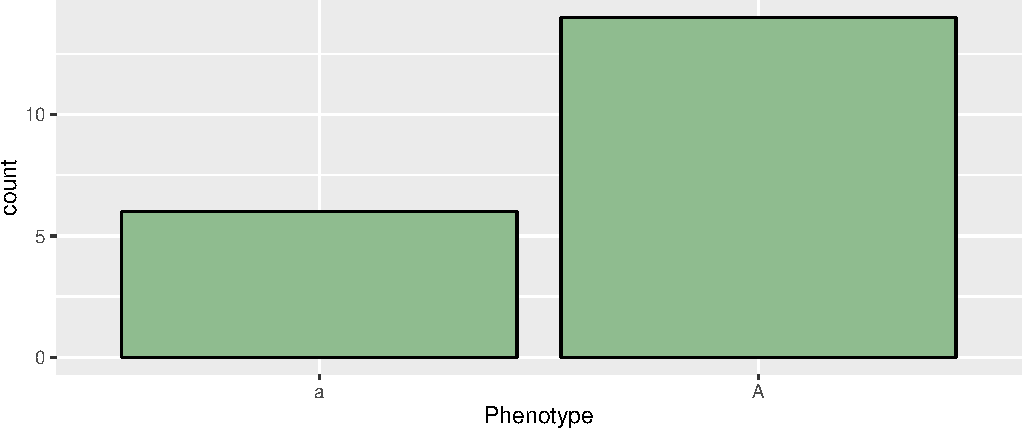
\includegraphics{skeleton_files/figure-latex/unnamed-chunk-77-1.pdf}

Next you enter the Hypothesized Probabilities \texttt{p}, such as 0.75
and 0.25 for a predicted Mendelian 3:1 ratio of A to a phenotypes from a
Aa X Aa cross. Notice the order here matters so we designate 0.25 first
and then 0.75 since \texttt{a} came before \texttt{A} in our table.

\begin{Shaded}
\begin{Highlighting}[]
\KeywordTok{chisq.test}\NormalTok{(phen_cont, }\DataTypeTok{p =} \KeywordTok{c}\NormalTok{(}\FloatTok{0.25}\NormalTok{, }\FloatTok{0.75}\NormalTok{))}
\end{Highlighting}
\end{Shaded}

\begin{Verbatim}[frame=single]

    Chi-squared test for given probabilities

data:  phen_cont
X-squared = 0.26667, df = 1, p-value = 0.6056
\end{Verbatim}

The \texttt{p-value} here is used to decide if the null hypothesis can
be rejected.

Summary statement:

\begin{quote}
The observed phenotypic ratio was not significantly different from the
expected ratio of 3:1 for a one-gene, two-allele, simple dominance
Mendelian model (Chi-Square, X\textsuperscript{2} = 0.27, df = 1, p =
0.61).
\end{quote}

See page I-13 for more explanation.

%\addtocontents{toc}{\protect\mbox{}\protect\hfill\par}
%\addtocontents{toc}{\protect\vfill}
\addtocontents{toc}{\protect\clearpage}

\end{document}
